\documentclass{article}
\usepackage{graphicx, amsfonts, amsmath, amssymb, amsthm, cancel, braket} % Required for inserting images

\title{Metodi Matematici della Fisica}
\author{mathcal notes}
\date{January 2026}

\begin{document}

\maketitle
\tableofcontents
\newpage

\section{Spazi e operatori lineari}
\subsection{Spazi lineari}
\textbf{Definizione:} un $\mathbf{K}$-spazio lineare $L$ è un insieme su cui sono definite due operazioni: somma e prodotto per scalare
\begin{gather}
    + : L \times L \longrightarrow L \qquad \cdot : \mathbf{K} \times L \longrightarrow \mathbf{K} \notag
\end{gather}
che soddisfano le seguenti proprietà per ogni $u, v, w \in L$ e ogni $\alpha, \beta \in \mathbf{K}$
\begin{align}
    1. \qquad &u + (v + w) = (u + v) + w \notag \\
    2. \qquad & u + v = v + u \notag \\
    3. \qquad &\text{esiste } 0 \in L \text{ tale che } 0 + v = v + 0 = v \notag \\
    4. \qquad &\text{per ogni } v \in L \quad \text{ esiste } v' \in L \text{ tale che } v + v' = v' + v = 0 \notag \\
    5. \qquad &\alpha(u + v) = \alpha u + \alpha v \notag \\
    6. \qquad &(\alpha + \beta)u = \alpha u + \beta u \notag \\
    7. \qquad &\alpha(\beta u) = \beta(\alpha u) = (\alpha \beta) u \notag \\
    8. \qquad &1u = u \notag
\end{align}
\textbf{Definizione:} sia $L$ un $\mathbf{K}$-spazio lineare, $n$ vettori $v_1, \dots, v_n \in L$ sono detti linearmente dipendenti se esistono $c_1, \dots, c_n \in \mathbf{K}$ non nulli tali che
\begin{gather}
    c_1v_1 + \dots + c_nv_n = 0 \notag
\end{gather}
altrimenti sono detti linearmente indipendenti. \\ \\
\textbf{Definizione:} un $\mathbf{K}$-spazio vettoriale è detto $n$ dimensionale se ammette un insieme di $n$ vettori linearmente indipendenti e $n + 1$ vettori sono sempre linearmente dipendenti. \\ \\
\textbf{Definizione:} un insieme di $n$ vettori linearmente indipendenti in un spazio lineare $L$ $n$ dimensionale forma una base. \\ \\
\textbf{Teorema (1.1.1):} sia $L$ un $\mathbf{K}$-spazio lineare e sia $\{e_i : i = 1, \dots, n\}$ una base di $L$, allora per ogni $v \in L$ esistono unici $c_1, \dots, c_n \in \mathbf{K}$ tali che
\begin{gather}
    v = c_1e_1 + \dots + c_ne_n \notag
\end{gather}

\textbf{Dimostrazione:} poiché $L$ è uno spazio lineare $n$ dimensionale e $\{e_i : i = 1, \dots, n\}$ è un insieme di $n$ vettori linearmente indipendenti, essendo una base, si ha che esistono non nulli $a_0, \dots, a_n \in \mathbf{K}$ tali che
\begin{gather}
    a_0v + a_1e_1 + \dots + a_ne_n = 0 \notag
\end{gather}
con $a_0 \neq 0$. Allora segue che
\begin{gather}
    v = \sum_{i = 1}^n -\frac{a_i}{a_0}e_i \notag
\end{gather}
pertanto ponendo $c_i = -\frac{a_i}{a_0}$ si ha che
\begin{gather}
    v = \sum_{i = 1}^n c_ie_i \notag
\end{gather}
Dimostriamo ora che sono unici, supponiamo che esistano $c'_1, \dots, c'_n \in \mathbf{K}$ tali che
\begin{gather}
    v = c'_1e_1 + \dots + c'_ne_n \notag
\end{gather}
allora deve valere
\begin{gather}
    c_1e_1 + \dots + c_ne_n = c'_1e_1 + \dots c'_ne_n \notag
\end{gather}
e quindi
\begin{gather}
    (c_1 - c'_1)e_1 + \dots + (c_n - c'_n)e_n = 0 \notag
\end{gather}
ma allora $c_i - c'_i = 0$, ovvero $c_i = c'_i$ per ogni $i = 1, \dots, n$ poiché $\{e_i : i = 1, \dots, n\}$ è una base. \\ \\
\textbf{Definizione:} due spazi lineari $L_1$ e $L_2$ sono isomorfi se esiste $f : L_1 \longrightarrow L_2$ con $f$ isomorfismo, ovvero $f$ preserva la struttura di spazio lineare ed è biettiva. \\ \\
\textbf{Teorema (1.1.2):} tutti gli spazi lineari $n$ dimensionali sono tra loro isomorfi. \\

\textbf{Dimostrazione:} basta dimostrare che i $\mathbf{K}$-spazi lineari $n$ dimensionali sono isomorfi a $\mathbf{K}^n$. Sia $L$ un $\mathbf{K}$-spazio lineare $n$ dimensionale e sia $\{e_i : i = 1, \dots, n\}$ una base di $L$. Per ogni $v \in L$ esistono unici $c_1, \dots, c_n \in \mathbf{K}$ tali che
\begin{gather}
    v = \sum_{i = 1}^n c_ie_i \notag
\end{gather}
Consideriamo la seguente funzione lineare $f : L \longrightarrow \mathbf{K}^n$ definita da
\begin{gather}
    v \hookrightarrow (c_1, \dots, c_n) \notag
\end{gather}
Notiamo immediatamente che $f$ è un omomorfismo, infatti preserva la struttura di spazio lineare, è suriettiva poiché per ogni $(a_1, \dots, a_n) \in \mathbf{K}^n$ esiste $u \in L$ tale che
\begin{gather}
    u = \sum_{i = 1}^n a_ie_i \notag
\end{gather}
inoltre è iniettiva, infatti le coordinate rispetto ad una base sono uniche per ogni elemento di $L$, pertanto $f$ è un isomorfismo e $L \cong \mathbf{K}^n$. \\ \\
\textbf{Definizione:} un sotto spazio $L' \subset L$ è un sottospazio lineare se forma uno spazio lineare rispetto alle stesse operazioni di $L$. \\ \\
\textbf{Teorema (1.1.3):} sia $L$ un $\mathbf{K}$-spazio vettoriale, siano $E = \{e_i : i = 1, \dots, n\}$ e $E' = \{e'_i : i = 1, \dots, n\}$ due basi di $L$ tali che
\begin{gather}
    e_j = \sum_{i = 1}^n a_{ij}e'_i \notag
\end{gather}
e sia $v \in L$ tale che
\begin{gather}
    v = \sum_{i = 1}^n \mu_ie_i \notag \\
    v = \sum_{i = 1}^n \mu'_ie'_i \notag
\end{gather}
allora si ha che
\begin{gather}
    \mu_i = \sum_{j = 1}^n a_{ij}\mu'_j \notag \\
    \mu'_i = \sum_{j = 1}^n (a^{-1})_{ij}\mu_j \notag
\end{gather}

\textbf{Dimostrazione:} notiamo che
\begin{gather}
    v = \sum_{j = 1}^n\mu_je_j = \sum_{i, j = 1}^n\mu_ja_{ij}e'_i \notag
\end{gather}
dunque le coordinate di $v$ rispetto alla base $E'$ possono essere scritte come segue
\begin{gather}
    (\mu_1a_{11} + \dots + \mu_na_{1n}, \dots, \mu_1a_{n1} + \dots + \mu_na_{nn}) \notag
\end{gather}
poniamo $M = (a_{ij})_{ij}$ e indichiamo con $[v]_{B}$ il vettore (colonna) delle coordinate di $v$ rispetto ad una determinata base $B$ di $L$, allora si ha che
\begin{gather}
    [v]_{E'} = M[v]_E \notag
\end{gather}
inoltre $M$ è invertibile, infatti le sue colonne sono le coordinate degli elementi dalla base $E$ espressi in base $E'$ e poiché gli elementi della base sono linearmente indipendenti si ha $\det M \neq 0$, pertanto
\begin{gather}
    [v]_E = M^{-1}[v]_{E'} \notag
\end{gather}
ovvero la tesi.

\newpage
\subsection{Spazi lineari unitari}
\textbf{Definizione:} uno spazio lineare unitario e un $\mathbf{C}$-spazio lineare $L$ dotato di un prodotto interno
\begin{gather}
    (\cdot, \cdot) : L \times L \longrightarrow \mathbf{C} \notag
\end{gather}
che soddisfa le seguenti proprietà per ogni $u, v, w \in L$ e ogni $\alpha \in \mathbf{C}$
\begin{align}
    1. \qquad &(u, v) = (v, u)^* \notag \\
    2. \qquad &(u, v + w) = (u, v) + (u, w) \notag \\
    3. \qquad &(u, \alpha v) = \alpha(u, v) \notag \\
    4. \qquad &(u, u) \geq 0, \quad (u, u) = 0 \iff u = 0 \notag
\end{align}
\textbf{Osservazione:} dalla proprietà del prodotto interno segue che
\begin{align}
    - \qquad &(u + v, w) = (w, u + v)^* = (w, u)^* + (w, v)^* = (u, w) + (v, w) \notag \\
    - \qquad &(\alpha u, v) = (v, \alpha u)^* = \alpha(v, u)^* = \alpha^*(u, v) \notag
\end{align}
\textbf{Definizione:} in uno spazio lineare unitario $L$ è sempre possibile definire una norma
\begin{gather}
    \| \cdot \| : L \longrightarrow \mathbf{R}^+ \notag
\end{gather}
ponendo
\begin{gather}
    \|u\| = \sqrt{(u, u)} \notag
\end{gather}
per ogni $u \in L$. \\ \\
\textbf{Definizione:} in uno spazio lineare unitario $L$ è sempre possibile definire una relazione di ortogonalità ponendo
\begin{gather}
    u \perp v \iff (u, v) = 0 \notag
\end{gather}
per ogni $u, v \in L$. \\ \\
\textbf{Osservazione:} la norma induce una metrica, pertanto ogni spazio lineare unitario è anche uno spazio metrico. \\ \\
\textbf{Definizione:} una matrice $H = (h_{ij})_{ij}$ è detta matrice metrica di uno spazio lineare $L$ se soddisfa le seguenti proprietà
\begin{align}
    1. \qquad &H = H^\dagger \notag \\
    2. \qquad &\sum_{ij}\alpha^*_ih_{ij}\alpha_j \geq 0 \text{ per ogni } \alpha \in \mathbf{C}^n \notag
\end{align}
ovvero $H$ è hermitiana e definita positiva. \\ \\
\textbf{Proposizione (1.2.1):} sia $L$ uno spazio lineare unitario e sia $E = \{e_i : i = 1, \dots, n\}$ una base di $L$. Definire un prodotto interno è equivalente a definire una matrice metrica. \\

\textbf{Dimostrazione:} $(\rightarrow)$ sia $(\cdot, \cdot) : L \times L \rightarrow \mathbf{C}$ un prodotto interno definito su $L$. Poniamo
\begin{gather}
    h_{ij} = (e_i, e_j) \notag
\end{gather}
si ha che
\begin{align}
    h_{ij} &= (e_i, e_j) = (e_j, e_i)^* = h^*_{ji} \notag
\end{align}
inoltre
\begin{align}
    \sum_{ij}\alpha^*_ih_{ij}\alpha_j &= \sum_{ij}\alpha^*_i(e_i, e_j)\alpha_j \notag \\
    &= \sum_{ij} (\alpha_ie_i, \alpha_je_j) \notag \\
    &= \|\alpha\|^2 \geq 0 \notag
\end{align}
Pertanto $H = (h_{ij})_{ij}$ con $h_{ij} = (e_i, e_j)$ definisce una matrice metrica. \\
$(\leftarrow)$ Sia $H = (h_{ij})_{ij}$ una matrice metrica, definiamo
\begin{gather}
    (u, v) = \sum_{ij}u^*_ih_{ij}v_j \notag
\end{gather}
si verifica che tale definizione soddisfa tutte le proprietà di un prodotto scalare unitario, infatti per ogni $u, v, w \in L$ e ogni $\lambda \in \mathbf{C}$ si ha
\begin{align}
    1. \qquad &(v, u) = \sum_{ij}v^*_ih_{ij}u_j = (u, v)^* \notag \\
    2. \qquad &(u, v + w) = \sum_{ij}u^*_ih_{ij}(v_j + w_j) = (u, v) + (u, w) \notag \\
    3. \qquad &(u, \lambda v) = \sum_{ij}u^*_ih_{ij}\lambda v_j = \lambda\sum_{ij}u^*_ih_{ij}v_j = \lambda(u, v) \notag \\
    4. \qquad &(u, u) = \sum_{ij}u^*_ih_{ij}u_j \geq 0 \notag
\end{align}
\textbf{Definizione:} sia $L$ uno spazio lineare unitario, due vettori $u, v \in L$ sono detti mutualmente ortogonali se $(u, v) = 0$, in tal caso si scrive $u \perp v$. \\ \\
\textbf{Teorema (1.2.1):} in uno spazio lineare unitario $L$ è sempre possibile trovare una base ortonormale. \\

\textbf{Dimostrazione:} sia $E = \{e_i : i = 1, \dots, n\}$ una base di $L$ e sia $H = (h_{ij})_{ij}$ la matrice metrica definita dal prodotto interno di $L$. Definiamo
\begin{align}
    e'_1 &= e_1 \notag \\
    e'_2 &= \begin{vmatrix}
        h_{11} & h_{12} \\
        e_1 & e_2
    \end{vmatrix} = h_{11}e_2 - h_{12}e_1 \notag \\
    e'_k &= \begin{vmatrix}
        h_{11} & . & . & . & h_{1k} \\
        . & & & & . \\
        . & & & & . \\
        . & & & & . \\
        h_{k-1 \, 1} & . & . & . & h_{k-1 \, k} \\
        e_1 & & & & e_k
    \end{vmatrix} = \sum_{i = 1}^k e_i\mathrm{cof}_{ki}(H) \notag
\end{align}
verifichiamo che $E' = \{e'_i : i = 1, \dots, n\}$ sia un insieme di vettori mutualmente ortogonali
\begin{align}
    (e'_1, e'_2) &= h_{11}(e_1, e_2) - h_{12}(e_1, e_1) = h_{11}h_{12} - h_{12}h_{11} = 0 \notag
\end{align}
In generale per dimostrare che $(e'_i, e'_k) = 0$ per ogni $i = 1, \dots, k-1$ basta verificare che $(e_i, e'_k) = 0$ per ogni $i = 1, \dots, k-1$, infatti $e'_i$ è combinazione lineare di $e_1, \dots, e_i$. In particolare si ha
\begin{align}
    (e_i, e'_k) &= \sum_{j = 1}^k(e_i, e_j)\mathrm{cof}_{ji}(H) \notag \\
    &= \begin{vmatrix}
         h_{11} & . & . & . & h_{1k} \\
        . & & & & . \\
        . & & & & . \\
        . & & & & . \\
        h_{k-1 \, 1} & . & . & . & h_{k-1 \, k} \\
        h_{i1} & & & & h_{i \, k}
    \end{vmatrix} = 0 \notag
\end{align}
poiché è il determinante di una matrice con due righe uguali ($1 \leq i \leq k-1)$. A questo basta normalizzare gli stata, dunque poniamo
\begin{gather}
    f_i = \frac{e'_i}{\sqrt{(e'_i, e'_i)}} \notag
\end{gather}
e $F = \{f_i : i = 1, \dots, n\}$ forma una base ortonormale di $L$. \\ \\
\textbf{Proposizione (1.2.2):} sia $L$ uno spazio lineare unitario, sia $E = \{e_i : i = 1, \dots, n\}$ una base ortonormale di $L$ e sia $v = a_1e_1 + \dots + a_ne_n$ con $a_1, \dots, a_n \in \mathbf{C}$, allora per ogni $i = 1, \dots, n$ si ha che
\begin{gather}
    a_i = (e_i, v) \notag
\end{gather}

\textbf{Dimostrazione:} si ha che
\begin{align}
    (e_i, v) = \sum_{j = 1}^n a_j(e_i, e_j) = \sum_{i = 1}^n a_j\delta_{ij} = a_i \notag
\end{align}

\newpage
\subsection{Cambiamenti di base e matrici unitarie}
\textbf{Definizione:} una matrice $U \in \mathcal{M}_n(\mathbf{C})$ è detta unitaria se vale
\begin{gather}
    U^\dagger U = \mathbf{1} \notag
\end{gather}
\textbf{Osservazione:} sia $U$ una matrice unitaria, allora $|\det U| = 1$, infatti si ha
\begin{gather}
    1 = \det U^\dagger U = \det U^\dagger \det U = (\det U)^2 \notag
\end{gather}
\textbf{Proposizione (1.3.1):} sia $L$ uno spazio lineare unitario e siano $E = \{e_i : i = 1, \dots, n\}$ e $E' = \{e'_i : i = 1, \dots, n\}$ due basi ortonormali di $L$, allora si ha che la matrice di cambiamento di base da $E$ a $E'$ è unitaria. \\

\textbf{Dimostrazione:} scriviamo $e_j$ in termini della base $E'$
\begin{gather}
    e_j = \sum_{i = 1}^n \mu_{ij}e'_i \notag
\end{gather}
con $\mu_{ij} = (e'_i, e_j)$. La trasformazione inversa è data dalla matrice i cui coefficienti sono $\mu'_{ij} = (e_i, e'_j)$, dunque
\begin{gather}
    \mu_{ij} = (e'_i, e_j) = (e_j, e'_i)^* = \mu'^*_{ji} \notag
\end{gather}
pertanto si ottiene la tesi, ovvero $U^{-1} = U^\dagger$. \\ \\
\textbf{Osservazione:} se $A$ e $B$ sono matrici unitarie anche $C = AB$ è una matrice unitaria, infatti $C^\dagger = B^\dagger A^\dagger$ e $C^\dagger C = B^\dagger A^\dagger A B = \mathbf{1}$.

\newpage
\subsection{Funzionali lineari}
\textbf{Definizione:} sia $L$ un $\mathbf{K}$-spazio lineare, un funzionale lineare è una funzione
\begin{gather}
    f : L \longrightarrow \mathbf{K} \notag
\end{gather}
che soddisfa le seguenti proprietà per ogni $u, v \in L$ e ogni $\lambda \in \mathbf{K}$
\begin{align}
    1. \qquad &f(u + v) = f(u) + f(v) \notag \\
    2. \qquad &(f\lambda u) = \lambda f(u) \notag
\end{align}
Indichiamo con il simbolo $L^*$ l'insieme di tutti i funzionali lineare definiti da $L$ al campo $\mathbf{K}$, ovvero $L^* = \mathrm{Hom}(L, \mathbf{K})$, ed è detto spazio duale. \\ \\
Lo spazio duale $L^*$ forma uno spazio lineare rispetto alle seguenti operazioni di somma e prodotto per scalare
\begin{align}
    (f + g)(u) = f(u) + g(u) \qquad (\lambda f)(u) = \lambda f(u) \notag
\end{align}
per ogni $u, v \in L$ e ogni $\lambda \in \mathbf{K}$. \\ \\
\textbf{Teorema (1.4.1):} sia $L$ uno spazio lineare unitario tale che $\dim L = n < \infty$, si ha che $\dim L^* = n$ e $L \cong L^*$. \\

\textbf{Dimostrazione:} sia $\{e_i : i = 1, \dots, n\}$ una base di $L$, per ogni $i = 1, \dots, n$ definiamo $\phi_i \in L^*$ ponendo
\begin{gather}
    \phi_i(e_j) = \delta_{ij} \notag
\end{gather}
ed estensione lineare. Ogni $f \in L^*$ può essere scritta come combinazione lineare di $\phi_1, \dots, \phi_n$, infatti
\begin{align}
    f(u) = f(\sum_{i = 1}^n c_ie_i) &= \sum_{i = 1}^n c_if(e_i) \notag \\
    &= \sum_{i, j = 1}^n c_i\delta_{ij}f(e_i) \notag \\
    &= \sum_{i, j = 1}^n c_i\phi_i(e_j)f(e_i) \notag \\
    &= \sum_{i = 1}^n \lambda_i\phi(u) \notag
\end{align}
dove $\lambda_i = f(e_i) \in \mathbf{C}$ per ogni $i = 1, \dots, n$ e si è usata la linearità di $\phi_i$, infatti
\begin{gather}
    \sum_{i, j = 1}^n c_i\phi_i(e_j) = \sum_{i, j = 1}^n \phi_i(c_ie_j) = \sum_{i = 1}^n \phi_i(u) \notag
\end{gather}
Pertanto $\{\phi_i : i = 1, \dots, n\}$ è una base di $L^*$ (ogni insieme più piccolo non basterebbe a generare tutto $L^*$), quindi $\dim L^* = n$ e segue dal \textit{teorema (1.1.2)} che $L^* \cong \mathbf{C}^n$, dunque $L^* \cong L$. \\ \\
\textbf{Definizione:} la base $\{\phi_i : i = 1, \dots, n\}$ è detta base duale. \\ \\
\textbf{Teorema (di Riesz):} sia $L$ uno spazio lineare unitario, per ogni $\phi \in L^*$ esiste unico $\eta \in L$ tale che $\phi(u) = (\eta, u)$ per ogni $u \in L$. \\

\textbf{Dimostrazione:} sia $E = \{e_i : i = 1, \dots, n\}$ una base di $L$, fissiamo $\eta \in L$, si ha che la mappa $u \hookrightarrow (\eta, u)$ è un funzionale lineare, dunque è un elemento di $L^*$. Siano $\phi \in L^*$ e $\{\phi_i : i = 1, \dots, n\}$ la base duale, esistono unici $\lambda_1, \dots, \lambda_n \in \mathbf{C}$ tali che
\begin{gather}
    \phi(u) = \sum_{i = 1}^n \lambda_i\phi_i(u) \notag
\end{gather}
inoltre esistono unici $\mu_1, \dots, \mu_n \in \mathbf{C}$ tali che
\begin{gather}
    (\eta, u) = \sum_{i = 1}^n \mu_i\phi_i(u) \notag
\end{gather}
per far sì che $\phi(u) = (\eta, u)$ per ogni $u \in L$ dobbiamo scegliere $\eta$ tale che $\lambda_i = \mu_i$ per ogni $i = 1, \dots, n$. Sappiamo dal \textit{teorema 1.4.1} che
\begin{gather}
    \lambda_i = \phi(e_i) \qquad \mu_i = (\eta, e_i) \notag
\end{gather}
pertanto se $E$ è una base ortonormale basta scegliere
\begin{gather}
    \eta = (\phi(e_1), \dots, \phi(e_n)) \notag
\end{gather}
Altrimenti scrivendo $\eta$ come combinazione lineare degli elementi della base $E$
\begin{gather}
    \eta = \sum_{i = 1}^n x_ie_i \notag
\end{gather}
otteniamo
\begin{gather}
    (\eta, e_j) = \sum_{i = 1}^n x_i(e_i, e_j) = \sum_{i = 1}^n x_ih_{ij} \notag
\end{gather}
e quindi basta risolvere il seguente sistema lineare
\begin{gather}
    \begin{cases}
        \phi(e_1) = x_1h_{11} + \dots + x_nh_{n1} \\
        . \\
        . \\
        \phi(e_n) = x_1h_{1n} + \dots + x_nh_{nn}
    \end{cases} \notag
\end{gather}
con incognite $x_1, \dots, x_n \in \mathbf{C}$. Ovvero, in forma vettoriale si ha
\begin{gather}
    y = H^Tx \notag
\end{gather}
dove $y = (\phi(e_1), \dots, \phi(e_n))$. Essendo $H^T$ invertibile la soluzione è unica e si ha
\begin{gather}
    x = (H^T)^{-1}y \notag
\end{gather}
poniamo $\eta = x$, la tesi segue. \\ \\
Un altro modo per dimostrare il \textit{teorema di Riesz} è notando che $\dim \ker \phi = n - 1$, infatti $\dim \mathrm{Im} \, \phi \leq 1$ ($\dim \mathrm{Im} \, \phi = 0 \iff \phi = 0$). Sia $u \in \ker \phi$ e $\eta \in \ker^\perp \phi$, per ogni $v \in L$ esiste $\alpha \in \mathbf{C}$ tale che
\begin{gather}
    v = u + \alpha\eta \notag
\end{gather}
allora
\begin{gather}
    \phi(v) = \alpha\phi(\eta) \qquad (\eta, v) = \alpha\|\eta\|^2 \notag
\end{gather}
confrontando le due relazioni si ottiene
\begin{gather}
    \phi(v) = \frac{(\eta, v)}{\|\eta\|^2}\phi(\eta) = \left( \frac{\phi(\eta)^*}{\|\eta\|^2}\eta, u \right) = (\Tilde{\eta}, u) \notag
\end{gather}
Inoltre $\Tilde{\eta}$ è unico, infatti scelto un qualsiasi $\eta' \in \ker^\perp \phi$, $\eta' = \lambda \eta$ per qualche $\lambda \in \mathbf{C}$ si ha che
\begin{gather}
    \frac{\phi(\eta)^*}{\|\eta\|^2}\eta \rightarrow \frac{\lambda^*\phi(\eta)^*}{|\lambda|^2\|\eta^2\|}\lambda\eta = \frac{\phi(\eta)^*}{\|\eta\|^2}\eta \notag
\end{gather}
dunque si ottiene la tesi.

\newpage
\subsection{Polinomi ortonormali}
\textbf{Definizione:} poniamo $P^{k-1}_\mathbf{C}[x]$ l'insieme dei polinomi di grado $n \leq k-1$, definiti su un intervallo $(a, b) \subset \mathbf{R}$ a coefficienti complessi. \\ \\
Per ogni scelta di prodotto interno $(\cdot, \cdot)$ in $P_{k-1}[x]$ è possibile trovare una base ortonormale di polinomi (segue dal \textit{teorema 1.2.1}). Un esempio di prodotto scalare è dato da
\begin{gather}
    (p, q) = \int_a^b \omega(x)p^*(x)q(x) \, dx \notag
\end{gather}
per ogni $p, q \in P^{k-1}_\mathbf{C}[x]$. Il termine $\omega(x)$ è detto peso, ovvero una funzione positiva quasi ovunque in $(a, b)$. \\ \\
La base standard per $P^{k-1}_\mathbf{C}[x]$ è
\begin{gather}
    S = \{1, x, x^2, \dots, x^{k-1}\} \notag
\end{gather}
in questo caso la matrice metrica è data da
\begin{gather}
    h_{ij} = \int_a^b \omega(x)x^{i + j} \, dx = \omega_{i + j} \notag
\end{gather}
Possiamo sempre assumere che $\omega$ sia normalizzata in $(a, b)$, ovvero
\begin{gather}
    1 = \int_a^b \omega(x) \, dx \notag
\end{gather}
Usando la base $S$ possiamo costruire una base ortonormale seguendo il procedimento del \textit{teorema 1.2.1}. \\ \\
Poniamo $P^k_\mathbf{R}[x]$ lo spazio dei polinomi di grado $n \leq k$, definiti su un intervallo $(a, b) \subset \mathbf{R}$ a coefficienti reali. Definiamo il seguente prodotto scalare
\begin{gather}
    (p, q) = \int_a^b \omega(x)p(x)q(x) \, dx \notag
\end{gather}
per ogni $p, q \in P^k_\mathbf{R}[x]$. \\ \\
\textbf{Teorema (1.5.1):} sia $\{p_n : n = 0, \dots, k\}$ una base ortonormale di $P^k_\mathbf{R}[x]$, allora per ogni $n = 1, \dots, k$ si ha che $p_n(x)$ ha $n$ radici reali e distinti. \\

\textbf{Dimostrazione:} si ha che $p_0(x) = 1$, dunque $p_0$ non ha radici. Per ipotesi si ha che
\begin{gather}
    \int_a^b \omega(x)p_0(x)p_n(x) \, dx = 0 \notag
\end{gather}
per ogni $n = 1, \dots, k$. Il peso $\omega$ è positivo quasi ovunque in $(a, b)$ pertanto $p_n$ deve cambiare segno almeno una volta in $(a, b)$ per far sì che l'integrale sia nullo. Poiché $p_n$ è continuo in $(a, b)$ per il teorema degli zeri si ha che $p_n$ ha almeno una radice in $(a, b)$. \\
Siano $x_1, \dots, x_m$ la radici di $p_n$ con molteplicità dispari in $(a, b)$, ovviamente si ha $m \leq n$, altrimenti $p_n$ sarebbe di grado maggiore di $n$. Poniamo
\begin{gather}
    q(x) = (x-x_1)\cdot \dots \cdot(x-x_m) \notag
\end{gather}
e definiamo il seguente polinomio
\begin{gather}
    p(x) = p_n(x)q(x) \notag
\end{gather}
Le radici di $p$ in $(a, b)$ sono $x_1, \dots, x_m$ e hanno molteplicità pari. Dunque $p$ non cambia mai segno in $(a, b)$, segue che
\begin{gather}
    (p_n, q) = \int_a^b \omega(x)p_n(x)q(x) \, dx \neq 0 \notag
\end{gather}
Possiamo esprimere $q$ come combinazione lineare dei primi $m$ polinomi della base ortonormale, ovvero
\begin{gather}
    q(x) = \sum_{j = 0}^m a_jp_j(x) \notag
\end{gather}
per qualche $a_1, \dots, a_m \in \mathbf{R}$. Segue che
\begin{gather}
    (p_n, q) = \sum_{j = 0}^m a_j(p_n, p_j) \neq 0 \notag
\end{gather}
ciò vale per ogni $n = 1, \dots, k$ (fissato). In particolare i termini con $0 \leq j \leq n-1$ sono nulli, deve per forza valere $m = n$ per far sì che ci sia un contributo non nullo, ovvero $(p_n, p_n)$. \\ \\
\textbf{Teorema (1.5.2):} sia $\{p_n : n = 0, \dots, k\}$ una base ortonormale di $P^k_\mathbf{R}$. Allora per $j < k$, $j$ fissato, vale la seguente relazione di ricorrenza
\begin{gather}
    xp_j(x) = a_jp_{j+1}(x) + b_jp_j(x) + c_jp_{j-1}(x) \notag
\end{gather}

\textbf{Dimostrazione:} poiché abbiamo fissato $j < k$ si ha che $xp_j \in P^k_\mathbf{R}$, pertanto lo possiamo esprimere come combinazione lineare degli elementi della base ortonormale
\begin{gather}
    xp_j(x) = \sum_{i = 0}^k \alpha_{ij}p_i(x) \notag
\end{gather}
dove
\begin{gather}
    \alpha_{ij} = (p_i, xp_j) \notag
\end{gather}
tuttavia si ha
\begin{gather}
    (p_i, xp_j) = \int_a^b \omega(x)p_i(x)xp_j(x) \, dx = 0 \notag
\end{gather}
se e solo se il grado di $xp_j$ è inferiore del grado di $p_i$, ovvero se e solo se $j + 1 < i$, infatti essendo $xp_j$ un polinomio di grado $j + 1$ è un elemento del sottospazio lineare $P^{j + 1}_\mathbf{R}$. Segue che $\alpha_{ij} \neq 0$ se e solo se $i \leq j + 1$. Inoltre si ha
\begin{align}
    (p_i, xp_j) = (xp_i, p_j) \notag
\end{align}
dunque deve valere anche $i \geq j - 1$ per far sì che $a_{ij} \neq 0$, pertanto ponendo
\begin{gather}
    a_j = \alpha_{j + 1 \, j} \quad b_j = \alpha_{jj} \quad c_j = \alpha_{j - 1 \, j} \notag
\end{gather}
si ottiene la tesi. \\ \\
\textbf{Teorema (1.5.3):} sia $\{p_n : n = 0, \dots, k\}$ una base ortonormale di $P^k_\mathbf{R}$ con $(a, b) = (-b, b)$ e con pesi pari, ovvero $\omega(-x) = \omega(x)$ per ogni $x \in (-b, b)$. Segue che $p_n(-x) = (-1)^np_n(x)$ per ogni $x \in (-b, b)$. \\

\textbf{Dimostrazione:} si ha $p_0(x) = 1$ per ogni $x \in (-b, b)$, dunque è pari, $p_1$ è della forma
\begin{gather}
    p_1(x) = \alpha + \beta x \notag
\end{gather}
imponendo $(p_0, p_1) = 0$ si ottiene
\begin{gather}
    0 = (p_0, p_1) = \int_{-b}^b \omega(x)(\alpha + \beta x) \, dx = \alpha\omega_0 \notag
\end{gather}
dunque $\alpha = 0$ e $p_1(x) = \beta x$ e quindi dispari. Analogamente $p_2$ è della forma
\begin{gather}
    p_2(x) = \Tilde{\alpha} + \tilde{\beta} x + \tilde{\gamma} x^2 \notag
\end{gather}
imponendo $(p_1, p_2) = 0$ si ottiene
\begin{gather}
    0 = (p_1, p_2) = \int_{-b}^b \omega(x)\beta x(\tilde{\alpha} + \tilde{\beta}x + \tilde{\gamma}x^2) \, dx = \beta\tilde{\beta}\omega_2 \notag
\end{gather}
dunque $\tilde{\beta} = 0$ e $p_2(x) = \tilde{\alpha} + \tilde{\gamma}x^2$ e quindi pari. Per il \textit{teorema 1.5.2} possiamo scrivere
\begin{gather}
    xp_1 = a_1p_2 + b_1p_1 + c_1p_0 = a_1(\tilde{\alpha} + \tilde{\gamma}x^2) + b_1\beta x + c_1 \notag
\end{gather}
poiché $xp_1$ deve essere pari si ha che $b_1 = 0$. Ragionando per induzione, supponiamo che sia vero per $xp_{j-1}$, ovvero $b_{j-1} = 0$ e $xp_{j-1}$ con parità $(-1)^{j}$, e dimostriamo che vale anche per $j$. Per il \textit{teorema 1.5.2} possiamo scrivere
\begin{gather}
    xp_j = a_jp_{j+1} + b_jp_j + c_jp_{j-1} \notag
\end{gather}
facendo il prodotto scalare con $p_j$ si ha
\begin{gather}
    0 = (p_j, xp_j) = a_j(p_j, p_{j+1}) + b_j(p_j, p_j) + c_j(p_j, p_{j-1}) = b_j \notag
\end{gather}
il termine $(p_j, xp_j) = 0$ perché è l'integrale di una funzione dispari su un intervallo simmetrico rispetto all'origine, infatti l'ipotesi induttiva su $j-1$ comprende che per $k = j-2, j - 1, j$ si abbia $p_k(-x) = (-1)^kp_k(x)$. Segue che
\begin{gather}
    xp_j = a_jp_{j+1} + c_jp_{j-1} \notag
\end{gather}
notiamo che
\begin{gather}
    a_jp_{j+1} = xp_j - c_jp_{j-1} \notag
\end{gather}
sappiamo che $xp_j$ ha parità $(-1)^{j+1}$ e $p_{j-1}$ ha parità $(-1)^{j-1}$, ma
\begin{gather}
    (-1)^{j+1} = (-1)^2(-1)^{j-1} = (-1)^{j-1} \notag
\end{gather}
dunque $p_{j+1}$ ha parità $(-1)^{j+1}$ e si ottiene la tesi.

\subsubsection{Polinomi classici}
Per i polinomi classici (Hermite, Legendre, Laguerre...) vale la formula di Rodriguez, ovvero
\begin{gather}
    r_n(x) = \frac{1}{\omega(x)}\left(\frac{d^n}{dx^n}\omega(x)\sigma^n(x)\right) \notag
\end{gather}
dove $\sigma$ è un polinomio. La funzione generatrice dei polinomi è data da
\begin{gather}
    \phi(x, t) = \sum_{n = 0}^\infty \frac{1}{n!}r_n(x)t^n \notag
\end{gather}
\textbf{Polinomi di Hermite $(H_n)$:} sono caratterizzati da
\begin{gather}
    \omega(x) = \frac{1}{\sqrt{\pi}}e^{-x^2} \qquad (a, b) = (-\infty, \infty) \quad \sigma(x) = -1 \notag \\
    r_n(x) = H_n(x) \longrightarrow H_n(x) = (-1)^ne^{-x^2}\frac{d^n}{dx^n}e^{-x^2} \notag \\
    \phi(x, t) = \sum_{n = 0}^\infty \frac{H_n(x)}{n!}t^n = e^{(-(x - t)^2 + x^2)} \notag
\end{gather}
\textbf{Polinomi di Legendre $(P_n)$:} sono caratterizzati da
\begin{gather}
    \omega(x) = \frac{1}{2} \quad (a, b) = (-1, 1) \quad \sigma(x) = \frac{1}{2}(x^2 - 1) \notag \\
    r_n(x) = n!P_n(x) \longrightarrow P_n(x) = \frac{1}{n!}\frac{d^n}{dx^n}\frac{(x^2 - 1)}{4} \notag \\
    \phi(x, t) = \sum_{n = 0}^\infty P_n(x)t^n = (1 -2xt + t^2)^{-1/2} \notag
\end{gather}
\textbf{Polinomi di Laguerre $(L^\alpha_n)$:} sono caratterizzati da
\begin{gather}
    \omega(x) = x^\alpha e^{-x} \quad (a, b) = (0, \infty) \quad \sigma(x) = x \quad (\alpha \in \mathbf{Z}, \alpha > -1) \notag \\
    r_n(x) = n!L^\alpha_n(x) \longrightarrow L^\alpha_n(x) = \frac{1}{n!}x^\alpha e^{-x}\frac{d^n}{dx^n}x^{\alpha + n}e^{-x} \notag \\
    \phi(x, t) \sum_{n = 0}^\infty L^\alpha_n(x)t^n = \frac{1}{(1-t)^{\alpha + 1}}e^{\frac{xt}{t-1} \notag}
\end{gather}
\textbf{Polinomi di Chebyshev $(T_n(x))$:} soddisfano la relazione di ricorrenza
\begin{gather}
    T_0(x) = 1, \quad T_1(x) = x, \quad T_{n+1}(x) = 2xT_n(x) - T_{n-1}(x) \notag
\end{gather}
inoltre soddisfano
\begin{gather}
    \int_{-1}^1 \frac{1}{\sqrt{1 - x^2}}\frac{2}{\pi}T_n(x)T_m(x) = \delta_{nm} \notag
\end{gather}

\newpage
\subsection{Operatori lineari}
\textbf{Definizione:} siano $L$ e $L'$ $\mathbf{C}$-spazi lineari, un operatore lineare è una mappa $A : L \longrightarrow L'$ che soddisfa le seguenti proprietà per ogni $u, v \in L$ e ogni $\lambda \in \mathbf{C}$
\begin{align}
    1. \qquad &A(u + v) = A(u) + A(v) \notag \\
    2. \qquad &A(\lambda u) = \lambda A(u) \notag
\end{align}
in generale verranno considerati endomorfismi $A : L \longrightarrow L$. \\ \\
\textbf{Teorema (1.6.1):} sia $L$ un $\mathbf{C}$-spazio lineare e sia $E = \{e_i : i = 1, \dots, n\}$ una base di $L$, un operatore lineare $A$ è univocamente determinato dalla sua azione sugli elementi della base. \\

\textbf{Dimostrazione:} sia $u \in L$, esprimiamo $u$ in termini della base $E$, si ha
\begin{gather}
    u = a_1e_1 + \dots + a_ne_n \notag
\end{gather}
per qualche $a_1, \dots, a_n \in \mathbf{C}$. Osserviamo che
\begin{gather}
    A(u) = A(\sum_{i = 1}^n a_ie_i) = \sum_{i = 1}^n a_iA(e_i) \notag
\end{gather}
poniamo $\omega_i = A(e_i) \in L$. Note le coordinate $\lambda_1, \dots, \lambda_n$ rispetto alla base $E$ di un qualsiasi vettore $v \in L$, si ha che
\begin{gather}
    A(v) = \sum_{i = 1}^n \lambda_i\omega_i \notag
\end{gather}
\textbf{Teorema (1.6.2):} sia $L$ un $\mathbf{C}$-spazio lineare, sia $E = \{e_i : i = 1, \dots, n\}$ una base di $L$ e sia $A$ un operatore lineare. Poniamo $\omega_j = A(e_j)$, in termini della base $E$ si ha
\begin{gather}
    \omega_j = \sum_{i = 1}^n a_{ij}e_i \notag
\end{gather}
allora $A$ è univocamente determinato dalla matrice $(a_{ij})_{ij}$ e agisce da sinistra su vettori colonna. \\

\textbf{Dimostrazione:} sia $v \in L$, in termini della base $E$ si ha
\begin{gather}
    v = \sum_{i = 1}^n \lambda_ie_i \notag
\end{gather}
per qualche $\lambda_1, \dots, \lambda_n \in \mathbf{C}$. Indichiamo con $[v]_E$ la $n$-upla di $\mathbf{C}^n$ che ha come $i$-esima componente $\lambda_i$, per ogni $i = 1, \dots, n$. Sappiamo, dal \textit{teorema 1.6.1}, che
\begin{gather}
    A(v) = \sum_{j = 1}^n \lambda_j\omega_j = \sum_{i, j = 1}^n \lambda_ja_{ij}e_i \notag
\end{gather}
ovvero
\begin{align}
    [v]_E &= \begin{pmatrix}
        \lambda_1a_{11} + \dots + \lambda_na_{1n} \\
        . \\
        . \\
        \lambda_{1}a_{n1} + \dots + \lambda_na_{nn}
    \end{pmatrix} \notag \\
    &= \begin{pmatrix}
        a_{11} & . & . & a_{1n} \\
        . & & & . \\
        . & & & . \\
        a_{n1} & . & . & a_{nn}
    \end{pmatrix}
    \begin{pmatrix}
        \lambda_1 \\
        . \\
        . \\
        \lambda_n
    \end{pmatrix} \notag
\end{align}
dunque, identificando $L$ con $\mathbf{C}^n$ come dimostrato nel \textit{teorema 1.1.2}, possiamo identificare l'azione di $A$ su $v$ con la moltiplicazione riga per colonna tra la matrice $(a_{ij})_{ij}$ e la $n$-upla $[v]_E$. \\ \\
\textbf{Corollario:} se la base $E$ è ortonormale si ha che $a_{ij} = (e_i, A(e_j))$, infatti $a_{ij}$ non è altro che la $i$-esima coordinata di $A(e_j)$ rispetto alla base $E$. \\ \\
\textbf{Definizione:} la matrice $(a_{ij})_{ij}$ è detta matrice rappresentativa di $A$. Nel caso generale in cui $A : L \longrightarrow L'$, per qualche $L, L'$ spazi lineari, indichiamo con
\begin{gather}
    M^E_{E'}(A) \notag
\end{gather}
dove $E$ è una base di $L$ ed $E'$ un base di $L'$, la matrice rappresentativa di $A$. \\ \\
\textbf{Teorema (1.6.3):} sia $L$ un $\mathbf{C}$-spazio lineare, sia $A : L \longrightarrow L$, siano $E = \{e_i : i = 1, \dots, n\}$ e $E' = \{e'_i : i = 1, \dots, n\}$ basi di $L$. Allora esiste unica $S \in \mathcal{M}_n(\mathbf{C})$ tale che
\begin{gather}
    M^{E'}_{E'}(A) = S^{-1} M^E_E(A) S \notag
\end{gather}

\textbf{Dimostrazione:} si ha che $M^E_E(A) = (a_{ij})_{ij}$ con $a_{ij}$ definito da
\begin{gather}
    A(e_j) = \sum_{i = 1}^na_{ij}e_i \notag
\end{gather}
Poniamo $M^{E'}_{E'}(A) = (a'_{ij})_{ij}$ con $a'_{ij}$ definito da
\begin{gather}
    A(e'_j) = \sum_{i = 1}^na'_{ij}e'_i \notag
\end{gather}
esprimiamo gli elementi della base $E$ in termini della base $E'$, ovvero
\begin{gather}
    \begin{cases}
        e_1 = \sum_{i = 1}^n s_{i1}e'_i \\
        . \\
        . \\
        e_n = \sum_{i = 1}^n s_{in}e'_i
    \end{cases} \notag
\end{gather}
si ha che
\begin{gather}
    A(e'_j) = A(\sum_{i = 1}^n s^{(-1)}_{ij}e_i) = \sum_{i = 1}^ns^{(-1)}_{ij}A(e_i) = \sum_{i, k = 1}^n s^{(-1)}_{ij}a_{ki}e_k = \sum_{i, k, l = 1}^n s^{(-1)}_{ij}a_{ki}s_{lk}e'_l \notag
\end{gather}
ovvero
\begin{gather}
    M^{E'}_{E'}(A) = S^{-1}M^E_E(A)S \notag
\end{gather}
con $S = (s_{ij})_{ij}$ matrice di cambiamento di base da $E$ a $E'$. \\ \\
\textbf{Corollario:} il determinante di due matrici simili, ovvero legate da una relazione del tipo
\begin{gather}
    A = S^{-1}BS \notag
\end{gather}
è uguale. \\ \\
\textbf{Teorema (1.6.4):} sia $L$ un $\mathbf{C}$-spazio lineare e sia $A \in \mathrm{Hom}(L, L)$, allora $A$ ammette almeno un autovalore, con relativo autovettore. \\

\textbf{Dimostrazione:} vogliamo risolvere $Av = \lambda v$ per $\lambda$ (e poi $v$ eventualmente). Passando alla matrice rappresentativa (rispetto ad una base qualsiasi $E$) ciò equivale a cercare $\lambda$ tale che
\begin{gather}
    (M^E_E(A) - \lambda\mathbf{1})v = 0 \notag
\end{gather}
ovvero
\begin{gather}
    \det(M^E_E(A) - \lambda\mathbf{1}) = 0 \rightarrow p(\lambda) = 0 \notag
\end{gather}
segue dal \textit{teorema fondamentale dell'algebra} che $p(\lambda)$ ammette almeno uno zero in $\mathbf{C}$, la tesi segue. \\ \\
\textbf{Teorema (1.6.5):} sia $L$ un $\mathbf{C}$-spazio lineare di dimensione $n$, si ha che $\mathrm{Hom}(L, L)$ ha dimensione $n^2$, inoltre è possibile definirvi un'algebra. \\

\textbf{Dimostrazione:} consideriamo una base $E = \{e_i : i = 1, \dots, n\}$ di $L$, a questo punto possiamo identificare $L$ con $\mathbf{C}^n$, allora qualsiasi operatore $A \in \mathrm{Hom}(L, L)$ è identificato con un unico elemento di $\mathcal{M}_n(\mathbf{C})$. Inoltre $\mathcal{M}_n(\mathbf{C}) \cong \mathbf{C}^{n^2}$, segue che $\mathrm{Hom}(L, L) \cong \mathbf{C}^n$, dunque $\dim \mathrm{Hom}(L, L) = n^2$. \\ \\
Definiamo un'algebra su $\mathrm{Hom}(L,L)$ introducendo l'operazione prodotto tra operatori come segue
\begin{gather}
    (A \cdot B)(u) = A(B(u)) \notag
\end{gather}
per ogni $A, B \in \mathrm{Hom}(L, L)$ e ogni $u \in L$, si verifica facilmente che il prodotto così definito è associativo e distributivo. Identificando $\mathrm{Hom}(L, L)$ con $\mathcal{M}_n(\mathbf{C})$ si ha che l'operazione prodotto tra operatori diventa l'operazione riga per colonna (da sinistra a destra) tra matrici $n \times n$. \\ \\
\textbf{Definizione:} sia $A \in \mathrm{Hom}(L, L)$, l'operatore aggiunto di $A$ è l'operatore $A^\dagger \in \mathrm{Hom}(L, L)$ che soddisfa la seguente relazione per ogni $u, v \in L$
\begin{gather}
    (u, A(v)) = (A^\dagger(u), v) \notag
\end{gather}
Tale definizione segue dal \textit{teorema di Riesz}, infatti per ogni $v$ fissato è possibile definire il seguente funzionale lineare
\begin{gather}
    \phi_v(u) = (u, A(v)) \notag
\end{gather}
sappiamo che esiste unico $\tilde{\phi}_v$ tale che
\begin{gather}
    \phi_v(u) = (\tilde{\phi}_v, v) \notag
\end{gather}
poniamo $\tilde{\phi}_v = A^\dagger(u)$. \\ \\
\textbf{Definizione:} un operatore $A \in \mathrm{Hom}(L, L)$ è detto
\begin{align}
    1. \qquad &\text{Autoaggiunto se } A = A^\dagger \notag \\
    2. \qquad &\text{Unitario se } A^{-1} = A^\dagger \notag \\
    3. \qquad &\text{Normale se } [A, A^\dagger] = 0 \notag
\end{align}
\textbf{Proposizione (1.6.1):} sia $L$ uno spazio lineare unitario, sia $E = \{e_i : i = 1, \dots, n\}$ una base ortonormale e sia $A \in \mathrm{Hom}(L, L)$ tale che $M^E_E(A) = (a_{ij})_{ij}$, allora si ha che $M^E_E(A^\dagger) = (b_{ij})_{ij}$ con $b_{ij} = a^*_{ji}$. Ovvero la rappresentazione matriciale di $A^\dagger$ è data dalla trasposta coniugata della rappresentazione matriciale di $A$. \\

\textbf{Dimostrazione:} sappiamo che
\begin{gather}
    a_{ij} = (e_i, A(e_j)) \notag
\end{gather}
pertanto
\begin{gather}
    a_{ij} = (e_i, A(e_j)) = (A^\dagger(e_i), e_j) = (e_j, A^\dagger(e_i))^* = b^*_{ji} \notag
\end{gather}

\newpage
\subsection{Funzioni di operatori lineari}
Una volta assegnata struttura di spazio vettoriale a $\mathrm{Hom}(L, L)$ è possibile definire polinomi di operatori, ovvero $p_n(A) \in \mathrm{Hom}(L, L)$ della forma
\begin{gather}
    p_n(A) = c_0\mathbf{1} + c_1A + \dots + c_nA^n \notag
\end{gather}
dove $A^k$ è il prodotto in $\mathrm{Hom}(L, L)$ di $k$ copie di $A$. \\ \\
Per funzioni analitiche intere è possibile definire la funzione di operatore tramite la serie di Taylor, sia $f$ una funzione complessa intera, definiamo
\begin{gather}
    f(A) = \sum_{n = 0}^\infty c_nA^n \notag
\end{gather}
dove $c_n$ è l'$n$-esimo coefficiente della serie di Taylor di $f$ in $\mathbf{C}$. \\ \\
\textbf{Definizione:} una mappa $\|\cdot\| : \mathrm{Hom}(L, L) \longrightarrow \mathbf{R}^+$ definisce una norma su $\mathrm{Hom}(L, L)$ se soddisfa le seguenti proprietà per ogni $A, B \in \mathrm{Hom}(L, L)$ e ogni $\lambda \in \mathbf{C}$
\begin{align}
    1. \qquad &\|A\| \geq 0 \notag \\
    2. \qquad &\|\lambda A\| = |\lambda|\|A\| \notag \\
    3. \qquad &\|A + B\| \leq \|A\| + \|B\| \notag
\end{align}
un esempio di norma è $\|\cdot\|_1$ data da
\begin{gather}
    \|A\|_1 = \sup_{v \in L}\frac{\|A(v)\|}{\|v\|} = \sup_{v \in L, \, \|v\| = 1}\|A(v)\| \notag
\end{gather}
dove la seconda uguaglianza è valida per la linearità dell'operatore $A$, infatti fissata una direzione data da un vettore $u$ si ha che
\begin{gather}
    \frac{\|A(\alpha u)\|}{\|\alpha u\|} = \frac{|\alpha|\|A(u)\|}{|\alpha|\|u\|} = \frac{\|A(u)\|}{\|u\|} \notag
\end{gather}
pertanto è lecito considerare solamente i versori dello spazio $L$. \\ \\
\textbf{Teorema (1.7.1):} sia $A \in \mathrm{Hom}(L, L)$ tale che la serie numerica
\begin{gather}
    \sum_{n = 0}^\infty |c_n|\|A\|^n \notag
\end{gather}
converge (assolutamente), allora
\begin{gather}
    \sum_{n = 0}^\infty c_nA^n \notag
\end{gather}
converge e
\begin{gather}
    \left\|\sum_{n = 0}^\infty c_nA^n\right\| \leq \sum_{n = 0}^\infty |c_n|\|A\|^n \notag
\end{gather}

\textbf{Dimostrazione:} poiché la serie numerica converge si ha che è di Cauchy, ovvero per ogni $\varepsilon > 0$ esiste $N \in \mathbf{N}$ tale che per ogni $n > m > N$ si ha
\begin{gather}
    \left|\sum_{k = 0}^n |c_k|\|A\|^k - \sum_{k = 0}^m |c_k|\|A\|^k\right| = \sum_{k = m}^n |c_k|\|A\|^k < \varepsilon \notag
\end{gather}
dalle proprietà $(2), (3)$ della norma segue che
\begin{gather}
    \left\|\sum_{k = m}^n c_kA^k\right\| \leq \sum_{k = m}^n |c_k|\|A\|^k < \varepsilon \notag
\end{gather}
dunque si ottiene la tesi.

\newpage
\subsection{Diagonalizzabilità di classi speciali di operatori lineari}
\textbf{Teorema (1.8.1):} gli operatori autoaggiunti hanno autovalori reali. \\

\textbf{Dimostrazione:} sia $A$ autoaggiunto e sia $v$ un autovettore (supponiamo normalizzato per semplicità) di $A$ con autovalore $\lambda$. Si ha che
\begin{align}
    A(v) &= \lambda v \notag
\end{align}
per ipotesi $A^\dagger = A$, pertanto
\begin{align}
    \lambda = (v, A(v)) = (A^\dagger(v), v) = (A(v), v) = (v, A(v))^* = \lambda^* \notag
\end{align}
quindi $\lambda^* = \lambda$, ovvero $\lambda \in \mathbf{R}$. \\ \\
\textbf{Corollario:} gli operatori anti-autoaggiunti, ovvero gli operatori $A$ tali che $A^\dagger = -A$, hanno autovalori immaginari puri. \\ \\
\textbf{Lemma (1.8.1):} ogni autospazio di $A$ è lasciato invariato da $B$ se $[A, B] = 0$. \\

\textbf{Dimostrazione:} sia $R_\lambda = \{v \in L : A(v) = \lambda v\}$ autospazio associato all'autovalore $\lambda$, sia $v \in R_\lambda$, allora
\begin{align}
    A(B(v)) = B(A(v)) = \lambda B(v) \notag
\end{align}
ovvero se $v \in R_\lambda$ si ha $B(v) \in R_\lambda$. \\ \\
\textbf{Teorema (1.8.2):} siano $A, B \in \mathrm{Hom}(L, L)$ tali che $[A, B] = 0$, allora ammettono almeno un autovettore in comune. \\

\textbf{Dimostrazione:} $A$ ammette almeno un autovalore $\lambda$, sia $R_\lambda$ l'autospazio di $A$ associato all'autovalore $\lambda$. Per il \textit{lemma 1.8.1} $R_\lambda$ è lasciato invariato da $B$. Sia $B'$ la restrizione di $B$ a $R_\lambda$, $B'$ ammette almeno un autovettore $v$. Per ipotesi $B'(v) = \lambda'v \in R_\lambda$, pertanto è combinazione lineare degli autovettori di $A$ in $R_\lambda$, quindi si $A(v) = \lambda v$. \\ \\
\textbf{Teorema (1.8.2):} ogni operatore autoaggiunto ammette una base ortonormale di autovettori. \\

\textbf{Dimostrazione:} sia $A$ autoaggiunto, dimostriamo che autovettori relativi a autovalori differenti di $A$ sono ortogonali. Siano $\lambda_1, \lambda_2$ autovalori di $A$ e siano $v_1, v_2$ gli autovettori associati. Si ha che
\begin{align}
    (v_1, A(v_2)) = \lambda_2(v_1, v_2) = \lambda_1(v_1, v_2) = (A(v_1), v_2) \notag
\end{align}
dato che per ipotesi $A^\dagger = A$. Pertanto deve valere
\begin{gather}
    (\lambda_1 - \lambda_2)(v_1, v_2) = 0 \notag
\end{gather}
poiché per ipotesi $\lambda_1 \neq \lambda_2$ si ha $(v_1, v_2) = 0$, ovvero $v_1 \perp v_2$. Se $A$ ammette $n$ autovalori distinti ammette una base ortonormale per quanto appena dimostrato (a meno di normalizzare i vettori). \\
Per il \textit{teorema fondamentale dell'algebra} $A$ ammette almeno un autovalore $\lambda$, sia $S_\lambda$ l'autospazio di $A$ associato all'autovalore $\lambda$. Consideriamo lo spazio ortogonale $S^\perp_\lambda$, $S^\perp_\lambda$ è lasciato invariato dall'azione di $A$, infatti se $v \in S_\lambda$ e $u \in S^\perp_\lambda$ si ha che
\begin{align}
    (v, A(u)) = (A(v), u) = \lambda(v, u) = 0 \notag
\end{align}
Consideriamo la restrizione $A'$ di $A$ su $S^\perp_\lambda$, $A'$ è ancora un operatore autoaggiunto e per il \textit{teorema fondamentale dell'algebra} ammette un almeno autovalore $\lambda'$ e dunque n autovettore in $S^\perp_\lambda$. Iterando questo processo si ottengono $n$ autovettori ortonormali (a meno di normalizzazione). \\ \\
\textbf{Teorema (1.8.3):} ogni operatore unitario ammette una base ortonormale di autovettori. \\

\textbf{Dimostrazione:} procedimento identico al \textit{teorema 1.8.2}, notando che gli operatori unitari $U$ lasciano invariati gli spazi ortogonali ai loro autospazi. \\ \\
\textbf{Teorema (1.8.4):} siano $A, B \in \mathrm{Hom}(L, L)$ operatori autoaggiunti, allora $[A, B] = 0$ se e solo se $A$ e $B$ ammettono una base ortonormale di autovettori in comune. \\

\textbf{Dimostrazione:} $(\rightarrow)$ per il \textit{teorema 1.8.3} $A$ e $B$ ammettono basi ortonormali di autovettori e per il \textit{teorema 1.8.1} uno di questi autovettori è in comune. Supponiamo, senza perdita di generalità, che sia $v_1$ e consideriamo lo spazio ortogonale a $v_1$, ovvero $S^\perp_{v_1}$. $S^\perp_{v_1}$ è lasciato invariato da $A$ e $B$, infatti se $u_1 \in S^\perp_{v_1}$ si ha che
\begin{align}
    (v_1, A(u_1)) &= (A(v_1), u_1) = a_1(v_1, u_1) = 0 \notag \\
    (v_1, B(u_1)) &= (B(v_1), u_1) = b_1(v_1, u_1) = 0 \notag
\end{align}
consideriamo la restrizione $A'$ e $B'$ di $A$ e $B$ a $S^\perp_{v_1}$, ovviamente si ha che $[A', B'] = 0$ e $A'$ e $B'$ sono autoaggiunti. Pertanto si può trovare un altro autovettore in comune e considerare lo spazio ortogonale a $v_1$ e $v_2$ e iterare il processo fino a trovare $n$ autovettori ortonormali (a meno di normalizzazione) in comune. \\ \\
$(\leftarrow)$ Se $A, B$ ammettono base ortonormale di autovettori in comune le loro matrici rappresentative in questa base sono diagonali e quindi commutano. \\ \\
\textbf{Teorema (1.8.5):} siano $A, B \in \mathrm{Hom}(L, L)$ operatori unitari, allora $[A, B] = 0$ se e solo se $A$ e $B$ ammettono una base ortonormale di autovettori in comune. \\

\textbf{Dimostrazione:} procedimenti identico al \textit{teorema 1.8.4}, notando che gli operatori unitari $U$ lasciano invariati gli spazi ortogonali ai loro autospazi. \\ \\
\textbf{Teorema (1.8.6):} $N \in \mathrm{Hom}(L, L)$ è un operatore normale se e solo se ammette una base ortonormale di autovettori. \\

\textbf{Dimostrazione:} $(\rightarrow)$ consideriamo i seguenti operatori
\begin{align}
    A_1 &= N + N^\dagger \notag \\
    A_2&= i(N - N^\dagger) \notag
\end{align}
notiamo che
\begin{align}
    A^\dagger_1 &= N^\dagger + N = N + N^\dagger = A_1 \notag \\
    A^\dagger_2 &= -i(N^\dagger - N) = i(N - N^\dagger) = A_2 \notag
\end{align}
dunque sono autoaggiunti e per ipotesi commutano poiché $[N, N^\dagger] = 0$, allora per il \textit{teorema 1.8.4} ammettono una base ortonormale di autovettori in comune. Allora anche
\begin{align}
    N &= \frac{1}{2}(A_1 - iA_2) \notag \\
    N^\dagger &= \frac{1}{2}(A_1 + iA_2) \notag
\end{align}
ammettono una base ortonormale di autovettori in comune, pertanto la tesi segue. \\ \\
$(\leftarrow)$ Sia $N$ diagonalizzabile in base ortonormale, allora la matrice rappresentativa di $N^\dagger$ nella stessa base non è altro che la trasposta coniugata, ovvero anche $N^\dagger$ è diagonale, quindi si ha $[N, N^\dagger] = 0$. \\ \\
\textbf{Teorema (1.8.7):} siano $A, B \in \mathrm{Hom}(L, L)$ operatori normali, allora $[A, B] = 0$ se e solo se $A$ e $B$ ammettono una base ortonormale di autovettori in comune. \\

\textbf{Dimostrazione:} $(\rightarrow)$ per il \textit{teorema 1.8.6} $A$ e $B$ ammettono basi ortonormali di autovettori e per il \textit{teorema 1.8.1} uno di questi autovettori è in comune. Supponiamo, senza perdita di generalità, che sia $v_1$ e consideriamo lo spazio ortogonale a $v_1$, ovvero $S^\perp_{v_1}$. $S^\perp_{v_1}$ è lasciato invariato da $A$ e $B$, infatti se $u_1 \in S^\perp_{v_1}$ si ha che
\begin{align}
    (v_1, A(u_1)) &= (A^\dagger(v_1), u_1) = a^*_1(v_1, u_1) = 0 \notag \\
    (v_1, B(u_1)) &= (B^\dagger(v_1), u_1) = b^*_1(v_1, u_1) = 0 \notag
\end{align}
consideriamo la restrizione $A'$ e $B'$ di $A$ e $B$ a $S^\perp_{v_1}$, ovviamente si ha che $[A', B'] = 0$ e $A'$ e $B'$ sono normali. Pertanto si può trovare un altro autovettore in comune e considerare lo spazio ortogonale a $v_1$ e $v_2$ e iterare il processo fino a trovare $n$ autovettori ortonormali (a meno di normalizzazione) in comune. \\ \\
$(\leftarrow)$ Se $A, B$ ammettono base ortonormale di autovettori in comune le loro matrici rappresentative in questa base sono diagonali e quindi commutano. \\ \\

\newpage
\subsection{Funzioni di operatori autoaggiunti}
Siano $\{A_1, \dots, A_l\}$ autoaggiunti tali che $[A_i, A_j] = 0$ per ogni $i, j = 1, \dots, l$. Poiché sono autoaggiunti e commutanti per il \textit{teorema 1.8.4} ammettono una base ortonormale di autovettori in comune, inoltre, dati $\lambda^{(k)}_{1}, \dots, \lambda^{(k)}_{m_k}$ autovalori di $A_k$ con $k = 1, \dots, l$, si ha che
\begin{align}
    A_k = \sum_{i = 1}^{m_k} \lambda^{(k)}_{i_k}E^{(k, 0)}_{i_k} \notag
\end{align}
ovvero $E^{(k, 0)}_{i_k} = 0$ per ogni $i_k = 1, \dots, m_k$. Gli operatori spettrali $E^{(k, 0)}_{i_k}$ sono polinomi di grado $m_k - 1 \leq n - 1$ in $A_k$, infatti si ha
\begin{align}
    E^{(k, 0)}_{i_k} &= \int_{C_\varepsilon(\lambda_i)}\frac{dz}{2\pi i}(z\mathbf{1} - A_k)^{-1} \notag \\
    &= \int_{C_\varepsilon(\lambda_i)}\frac{dz}{2\pi i}\frac{1}{\Delta^{(k)}_0(z)}\left(\left(\Delta^{(k)}_0(z)\mathbf{1} - \Delta^{(k)}_0(A_k)\right)(z\mathbf{1} - A_k)^{-1}\right) \notag
\end{align}
e poiché si ha $[A_i, A_j] = 0$ deve valere anche $[E^{(k, 0)}_{i_k}, E^{(k', 0)}_{j_{k'}}] = 0$. \\ \\
\textbf{Definizione:} sono detti proiettori composti i proiettori
\begin{gather}
    E^0_{i_1, \dots, i_l} = E^{(1, 0)}_{i_1} \cdot \dots \cdot E^{(l, 0)}_{i_l} \notag
\end{gather}
Dalle regole di commutazione dei proiettori dei singoli $A_k$ segue che
\begin{gather}
    E^0_{i_1, \dots, i_l} \cdot E^0_{j_1, \dots, j_l} = \delta_{i_1, j_1} \cdot \dots \cdot \delta_{i_l, j_l}E^0_{i_1, \dots, i_l} \notag
\end{gather}
\textbf{Definizione:} sia $f$ analitica in $D \subset \mathbf{C}^l$ tale che $\sigma(A_k) \subset D$ per ogni $k = 1, \dots, l$. Poniamo
\begin{gather}
    f(A_1, \dots, A_l) = \sum_{i_1, \dots, i_l}f(\lambda^{(1)}_{i_1}, \dots, \lambda^{(l)}_{i_l})E^0_{i_1, \dots, i_l} \notag
\end{gather}
\textbf{Definizione:} l'insieme $\{A_1, \dots, A_l\}$ si dice completo se ogni $E^0_{i_1, \dots, i_l} \neq 0$ proietta su uno spazio unidimensionale, ovvero non c'è degenerazione. \\ \\
\textbf{Teorema (1.9.1):} siano $\{A_1, \dots, A_l\}$ autoaggiunti commutanti e sia $B$ autoaggiunto tale che $[A_i, B] = 0$ per ogni $i = 1, \dots, l$. Allora se $\{A_1, \dots, A_l\}$ è completo si ha $B = f(A_1, \dots, A_l)$. \\

\textbf{Dimostrazione:} per ogni $l$-upla $(\lambda^{(1)}_{i_1}, \dots, \lambda^{(l)}_{i_l})$ esiste un unico autovettore comune ($i_k = 1, \dots, m_k$). Sia $\ket{\lambda^{(1)}_{i_1}, \dots, \lambda^{(l)}_{i_l}}$ tale che
\begin{gather}
    A_k\ket{\lambda^{(1)}_{i_1}, \dots, \lambda^{(l)}_{i_l}} = \lambda^{(k)}_{i_k}\ket{\lambda^{(1)}_{i_1}, \dots, \lambda^{(l)}_{i_l}} \notag
\end{gather}
Poiché $[A_i, B] = 0$ per ogni $i = 1, \dots, l$ si ha che $B$ lascia invariato ogni autospazio di $A_i$, per il \textit{teorema 1.8.1}, in particolare l'intersezione, tuttavia l'intersezione ha dimensione $1$ poiché per ipotesi $\{A_1, \dots, A_l\}$ forma un insieme completo, dunque l'intersezione è un autospazio di $B$, allora
\begin{gather}
    B\ket{\lambda^{(1)}_{i_1}, \dots, \lambda^{(l)}_{i_l}} = b(\lambda^{(1)}_{i_1}, \dots, \lambda^{(l)}_{i_l})\ket{\lambda^{(1)}_{i_1}, \dots, \lambda^{(l)}_{i_l}} \notag
\end{gather}
la tesi segue. \\ \\
\textbf{Definizione:} $\{B_1, \dots, B_l\}$ autoaggiunti sono detti irriducibili non lasciano invariato alcun sottospazio proprio dello spazio lineare su cui agiscono. \\ \\
\textbf{Teorema (di Schur):} sia $E \in \mathrm{Hom}(L, L)$ tale che $[E, B_i] = 0$ per ogni $i = 1, \dots, l$ con $\{B_1, \dots, B_l\} \subset \mathrm{Hom}(L, L)$ irriducibili, allora $E \propto \mathbf{1}$. \\

\textbf{Dimostrazione:} $E$ ammette almeno un autovalore $\lambda$ per il \textit{teorema fondamentale dell'algebra}, sia $S_\lambda$ l'autospazio di $E$ associato all'autovalore $\lambda$. Per il \textit{teorema 1.8.1} si ha che $B_i$ lascia invariato $S_\lambda$ per ogni $i = 1, \dots, l$. Allora, per definizione di insieme di operatori irriducibili, $S_\lambda = \mathbf{C}$, infatti non può essere l'insieme vuoto per definizione di autovettore, e quindi deve valere $E = \lambda\mathbf{1}$. \\ \\
\textbf{Teorema (di Lie - Trotter):} siano $A, B$ due generici operatori lineari, allora
\begin{gather}
    e^{A + B} = \lim_n (e^{A/n}e^{B/n})^n \notag
\end{gather}

\textbf{Dimostrazione:} dati $X, Y \in \mathrm{Hom}(L, L)$ si ha che
\begin{gather}
    X^n - Y^n = \sum_{k = 0}^{n - 1}X^k(X - Y)Y^{n - k - 1} \notag
\end{gather}
sia $t = 1/n$, allora, posto $S_t = e^{t(A + B)}$ e $T_t = e^{tA}e^{tB}$, verifichiamo che
\begin{align}
    \|S^n_t - T^n_t\| \rightarrow 0 \notag
\end{align}
per $n \rightarrow \infty$. Si ha che
\begin{align}
    \|S^n_t - T^n_t\| &\leq \sum_{k = 0}^{n - 1}\|S^k_t\|\|S_t - T_t\|\|T^{n - k - 1}_t\| \notag \\
    &= \|S_t - T_t\|\sum_{k = 0}^{n - 1}\|S^k_t\|\|T^{n - k - 1}_t\| \notag \\
    &\leq \|S_t - T_t\|\left[\max\left(\|S_t\|, \|T_t\|\right)\right]^{n - 1}\sum_{k = 0}^{n - 1}1 \notag \\
    &= n\|S_t - T_t\|\left[\max\left(\|S_t\|, \|T_t\|\right)\right]^n \notag \\
    &\leq n\|S_t - T_t\|\left(e^{(\|A\| + \|B\|)\frac{1}{n}}\right)^{n - 1} \rightarrow 0 \notag
\end{align}
per $n \rightarrow \infty$, infatti
\begin{align}
    \|S_t - T_t\| &= \left(\mathbf{1} + t(A + B) + \frac{t^2}{2}(A + B)^2 + o(t^2)\right) + \notag \\
    &\quad -\left(\mathbf{1} + tA + \frac{t^2}{2}A^2 + o(t^2)\right)\left(\mathbf{1} + tB + \frac{t^2}{2}B^2 + o(t^2)\right) \notag \\
    &= \frac{t^2}{2}[A, B] + o(t^2) \notag
\end{align}
sostituendo $t = 1/n$ si ottiene che $n\|S_{1/n} - T_{1/n}\| \rightarrow 0$ per $n \rightarrow \infty$. Mentre il termine esponenziale diventa costante per $n \rightarrow \infty$. \\ \\
\textbf{Teorema (Backer - Campbell - Hausdorff):} siano $A, B \in \mathrm{Hom}(L, L)$, allora $e^Ae^B = e^H$ con $H = A + B + \frac{1}{2}[A, B] + \frac{1}{12}\left([A, [A, B]] + [B, [B, A]]\right) + \dots$. \\

\textbf{Dimostrazione:} usando la definizione di esponenziale di matrice si ha
\begin{align}
    e^Ae^B &= \left(\mathbf{1} + A + \frac{1}{2}A^2 + \dots\right)\left(\mathbf{1} + B + \frac{1}{2}B^2 + \dots\right) \notag \\
    &= \mathbf{1} + (A + B) + \frac{1}{2}(A^2 + B^2) + AB + \dots \notag
\end{align}
sia $H = A + B + c_2AB + c'_2BA + p_2A^2 + p'_2B^2 + \dots$, allora si ha
\begin{align}
    e^H &= \mathbf{1} + H + \frac{1}{2}H^2 + \dots \notag \\
    &= \mathbf{1} + (A + B + c_2AB + c'_2BA + p_2A^2 + p'_2B^2) + \frac{1}{2}(\dots)^2 \notag \\
    &= \mathbf{1} + A + B + \left(c_2 + \frac{1}{2}\right)AB + \left(c'_2 + \frac{1}{2}\right)BA + \left(p_2 + \frac{1}{2}\right)A^2 + \left(p'_2 + \frac{1}{2}\right)B^2 \notag
\end{align}
dunque deve valere $c_2 = 1/2 = -c'_2$ e $p_2 = p'_2 = 0$. Pertanto si ottiene la tesi. \\ \\
\textbf{Osservazione:} se $[A, B] \propto \mathbf{1}$ si ha $H = A + B + \frac{1}{2}[A, B]$.




\newpage
\section{Analisi complessa}
\subsection{Funzioni complesse}
\textbf{Definizione:} una funzione complessa di variabile complessa è una mappa $f : D \subset \mathbf{C} \longrightarrow \mathbf{C}$ che associa ad ogni punto del piano complesso un punto dello stesso
\begin{gather}
    z \hookrightarrow \omega = f(z) \notag
\end{gather}
Poiché $f(z) \in \mathbf{C}$ ha una parte reale e una immaginaria, possiamo quindi scrivere
\begin{gather}
    f = \mathrm{Re}f + i\mathrm{Im}f \notag
\end{gather}
ovvero
\begin{gather}
    f(z) = f(x + iy) = u(x, y) + iv(x, y) \notag
\end{gather}
dove $u = \mathrm{Re}f$ e $v = \mathrm{Im}f$, $u, v : \mathbf{R}^2 \longrightarrow \mathbf{R}$. \\ \\
\textbf{Definizione:} sia $f : D \subset \mathbf{C} \longrightarrow \mathbf{C}$, sia $z_0$ un punto di accumulazione per $D$, si dice che
\begin{gather}
    \lim_{z \rightarrow z_0}f(z) = l \notag
\end{gather}
per qualche $l \in \mathbf{C}$, se per ogni $\varepsilon > 0$ esiste $\delta > 0$ tale che se
\begin{gather}
    |z - z_0| < \delta \notag
\end{gather}
si ha
\begin{gather}
    |f(z) - l| < \varepsilon \notag
\end{gather}
Considereremo in generale insiemi $R$ aperti connessi, detti regioni, e insiemi $D$ chiusi connessi, detti domini. \\ \\
\textbf{Definizione:} una funzione $f : D \longrightarrow \mathbf{C}$ è detta continua in $z_0 \in \partial D \cap D$ se per ogni $\varepsilon > 0$ esiste $\delta > 0$ tale che se
\begin{gather}
    |z - z_0| < \delta \notag
\end{gather}
si ha
\begin{gather}
    |f(z) - f(z_0)| < \varepsilon \notag
\end{gather}
ovvero se
\begin{gather}
    \lim_{z \rightarrow z_0}f(z) = f(z_0) \notag
\end{gather}
Se poniamo $f = u + iv$ per qualche $u, v : \mathbf{R}^2 \longrightarrow \mathbf{R}$, dire $f$ continua in $z_0 = x_0 + iy_0$ equivale a dire $u, v$ continue in $(x_0, y_0)$. \\ \\
\textbf{Definizione:} sia $f : D \longrightarrow \mathbf{C}$, $f$ è detta differenziabile in $z_0 \in \partial D \cap D$ se esiste $f_1 : D \longrightarrow \mathbf{C}$ continua in $z_0$ tale che
\begin{gather}
    f(z) = f(z_0) + (z - z_0)f_1(z) \notag
\end{gather}
se $f_1$ esiste è univocamente determinata da
\begin{gather}
    f_1(z) = \frac{f(z) - f(z_0)}{z - z_0} \notag
\end{gather}
e imponendo la continuità in $z_0$ si ottiene
\begin{gather}
    f_1(z_0) = \lim_{z \rightarrow z_0}\frac{f(z) - f(z_0)}{z - z_0} \notag
\end{gather}
$f_1(z_0)$ è detta derivata di $f$ in $z_0$ e viene indicata con i simboli
\begin{gather}
    \frac{df}{dz}(z_0) \quad \text{o} \quad f'(z_0) \notag
\end{gather}
\textbf{Osservazione:} se $f$ è differenziabile in $z_0$ si ha $f$ continua in $z_0$ (ma in generale non il viceversa), infatti
\begin{gather}
    \lim_{z \rightarrow z_0}|f(z) - f(z_0)| = \lim_{z \rightarrow z_0}|z - z_0||f'(z_0)| = 0 \notag
\end{gather}
\textbf{Esempio:} la funzione $z^n$, $n \in \mathbf{N}$, è differenziabile pre ogni $c \in \mathbf{C}$, infatti
\begin{gather}
    z^n = c^n + (z - c)f_1(z) \notag
\end{gather}
dove
\begin{gather}
    f_1(z) = z^{n - 1} + cz^{n - 2} + \dots + c^{n - 1} \notag
\end{gather}
segue che
\begin{gather}
    (z^n)' = nz^{n - 1} \notag
\end{gather}
Sia $f : D \longrightarrow \mathbf{C}$ e siano $u, v : \mathbf{R}^2 \longrightarrow \mathbf{R}$ tali che $f = u + iv$. Vediamo cosa comporta la scelta di incremento reale o puramente immaginario per la differenziabilità di $f$. Poniamo $z = x + iy \in \partial D \cap D$, sia $h$ reale, si ha che
\begin{align}
    \frac{df}{dz} &= \lim_{h \rightarrow 0}\frac{u(x + h, y) + iv(x + h, y) - u(x, y) -iv(x, y)}{h} \notag \\
    &= \lim_{h \rightarrow 0}\left[\frac{u(x + h, y) - u(x, y)}{h} + i\frac{v(x + h, y) - v(x, y)}{h}\right] \notag \\
    &= \frac{\partial u}{\partial x} + i\frac{\partial v}{\partial x} \notag
\end{align}
mentre scegliendo incremento puramente immaginario $ih$ si ha che
\begin{align}
    \frac{df}{dz} &= \lim_{h \rightarrow 0}\frac{u(x, y + h) + iv(x, y + h) - u(x, y) - iv(x, y)}{ih} \notag \\
    &= \lim_{h \rightarrow 0}\left(-i\frac{u(x, y + h) - u(x, y)}{h} + \frac{v(x, y + h) - v(x, y)}{h}\right) \notag \\
    &= -i\frac{\partial u}{\partial y} + \frac{\partial v}{\partial y} \notag
\end{align}
pertanto, affinché $\frac{df}{dz}$ esista in $D$ devono valere le condizioni di Cauchy - Riemann, ovvero
\begin{gather}
    \begin{cases}
        \frac{\partial u}{\partial x} = \frac{\partial v}{\partial y} \\
        \frac{\partial u}{\partial y} = -\frac{\partial v}{\partial x}
    \end{cases} \notag
\end{gather}
per ogni $z \in D$. \\ \\
\textbf{Teorema (condizione sufficiente per la differenziabilità):} sia $f : D \longrightarrow \mathbf{C}$, siano $u = \mathrm{Re}f$ e $v = \mathrm{Im}f$, allora una condizione sufficiente per la differenziabilità in $D$ è che $u, v$ siano di classe $C^1$ e soddisfino le condizioni di Cauchy - Riemann in $D$. \\

\textbf{Dimostrazione:} si ha che
\begin{align}
    \frac{df}{dz} &= \lim_{h, k \rightarrow 0}\frac{f(z + h + ik) - f(z)}{h + ik} \notag \\
    &= \lim_{h, k \rightarrow 0}\left(\frac{u(x + h, y + ik) - u(x, y)}{h + ik} + i\frac{v(x + h, y + ik) - v(x, y)}{h + ik}\right) \notag \\
    &= \lim_{h, k \rightarrow 0}\frac{1}{h + ik}\left(\frac{\partial u}{\partial x}h + \frac{\partial u}{\partial y}k + i\frac{\partial v}{\partial x}h + i\frac{\partial v}{\partial y}k\right) \notag \\
    &= \lim_{h, k \rightarrow 0}\frac{1}{h + ik}\left(\frac{\partial u}{\partial x}h - \frac{\partial v}{\partial x}k + i\frac{\partial v}{\partial x}h + i\frac{\partial u}{\partial x}k\right) \notag \\
    &= \lim_{h, k \rightarrow 0}\frac{1}{h + ik}(h + ik)\left(\frac{\partial u}{\partial x} + i\frac{\partial v}{\partial x}\right) \notag \\
    &= \frac{\partial u}{\partial x} + i\frac{\partial v}{\partial x} \notag
\end{align}
\textbf{Osservazione:} ponendo $f = u + iv$ possiamo trattare $f$ come una funzione di $z$ e $z^*$ sfruttando
\begin{gather}
    x = \frac{1}{2}(z + z^*) \qquad y = \frac{1}{2i}(z - z^*) \notag
\end{gather}
in tal caso si ha
\begin{align}
    \frac{df}{dz^*} &= \frac{\partial x}{\partial z^*}\frac{\partial f}{\partial x} + \frac{\partial y}{\partial z^*}\frac{\partial f}{\partial y} \notag \\
    &= \frac{1}{2}\left(\frac{\partial u}{\partial x} + i\frac{\partial v}{\partial x}\right) + \frac{i}{2}\left(\frac{\partial u}{\partial y} + i\frac{\partial v}{\partial y}\right) \notag \\
    &= \frac{1}{2}\left(\frac{\partial u}{\partial x} - \frac{\partial v}{\partial y}\right) + \frac{i}{2}\left(\frac{\partial u}{\partial y} + \frac{\partial v}{\partial x}\right) = 0 \notag
\end{align}
se $u, v$ soddisfano le condizioni di Cauchy - Riemann, pertanto la differenziabilità può essere anche vista come indipendenza da $z^*$. \\ \\
\textbf{Osservazione:} consideriamo le condizioni di Cauchy - Riemann per una coppia di funzioni $u, v$ di classe $C^2$
\begin{gather}
    \begin{cases}
        u_x = v_y \\
        u_y = -v_x
    \end{cases} \notag
\end{gather}
derivando rispetto a $x$ la prima e rispetto a $y$ la seconda si ha che
\begin{gather}
    \begin{cases}
        u_{xx} = v_{yx} \\
        u_{yy} = -v_{xy}
    \end{cases} \notag
\end{gather}
per il \textit{teorema di Schwartz} sappiamo che per una funzione $g : \mathbf{R}^2 \longrightarrow \mathbf{R}$ di classe $C^2$ vale
\begin{gather}
    g_{xy} = g_{yx} \notag
\end{gather}
pertanto si ottiene
\begin{gather}
    u_{xx} + u_{yy} = 0 \notag
\end{gather}
Facendo un ragionamento analogo per $v$ si ottiene
\begin{gather}
    v_{xx} + v_{yy} = 0 \notag
\end{gather}
ovvero $u, v$ sono funzioni armoniche. Pertanto una coppia di funzioni di classe $C^2$ che soddisfa le condizioni di Cauchy - Riemann forma anche una coppia di funzioni armoniche.

\newpage
\subsection{Singolarità}
\textbf{Definizione:} sia $f : D \longrightarrow \mathbf{C}$, un punto $z_0 \in \mathbf{C}$ è detto singolarità di $f$ se $f$ è non definita o non olomorfa in $z_0$. \\ \\
\textbf{Definizione:} sia $f : D \longrightarrow \mathbf{C}$ olomorfa, un punto $z_0 \in \mathbf{C}$ è detto singolarità isolata se esiste un intorno $I(\varepsilon, z_0)$ tale che $f$ è olomorfa in $I(\varepsilon, z_0) \setminus z_0$. Altrimenti $z_0$ è detta singolarità non isolata. \\ \\
Vediamo ora vari classi di singolarità isolate. Una singolarità $z_0$ di una funzione olomorfa $f$ è detta singolarità eliminabile se esiste finito il limite per $z \rightarrow z_0$ di $f(z)$, ovvero se
\begin{gather}
    \lim_{z \rightarrow z_0}f(z) = l \in \mathbf{C} \notag
\end{gather}
è detta polo (di ordine $n$) se esiste $n \in \mathbf{N}$ tale che in un intorno $I$ di $z_0$ vale
\begin{gather}
    f(z) = \frac{g(z)}{(z - z_0)^n} \notag
\end{gather}
con $g$ olomorfa per ogni $z \in I$. Infine $z_0$ è detta singolarità essenziale se non è né un polo né una singolarità eliminabile. \\ \\
\textbf{Proposizione (2.2.1):} sia $z_0 \in \mathbf{C}$, sia $\omega$ olomorfa in un intorno $I(r, z_0)$ e sia $\zeta$ olomorfa in un intorno $I(\rho, \omega_0) \subset \omega(I(r, z_0))$, dove $\omega_0 = \omega(z_0)$, allora $f(z) = \zeta(\omega(z))$ è olomorfa in $I(r, z_0)$. \\

\textbf{Dimostrazione:} per ipotesi esiste $\frac{d\omega}{dz}$ in un intorno di $z_0$ e $\frac{d\zeta}{dz}$ in un intorno di $\omega_0$, allora
\begin{align}
    f'(z_0) &= \lim_{z \rightarrow z_0}\frac{f(z) - f(z_0)}{z - z_0} \notag \\
    &= \lim_{z \rightarrow z_0}\frac{\zeta(\omega(z)) - \zeta(\omega(z_0))}{\omega(z) - \omega (z_0)}\frac{\omega(z) - \omega(z_0)}{z - z_0} \notag \\
    &= \zeta'(\omega(z_0))\omega'(z_0) \notag
\end{align}
dove si è usata la continuità di $\omega$.

\newpage
\subsection{Integrazione sul piano complesso}
Data una funzione $f : [a, b] \longrightarrow \mathbf{C}$ continua possiamo definire l'integrale di $f$ su $[a, b]$ come segue
\begin{gather}
    \int_a^b f(t) \, dt = \int_a^b \mathrm{Re}f(t) \, dt + i\int_a^b \mathrm{Im}f(t) \, dt \notag
\end{gather}
ovvero riconducendolo a integrali di funzioni reali. Dalla definizione data segue che per $f$ vale il \textit{teorema fondamentale del calcolo}. \\ \\
\textbf{Proposizione (2.3.1):} sia $f : [a, b] \longrightarrow \mathbf{C}$ una funzione continua, si ha che
\begin{gather}
    \left|\int_a^b f(t) \, dt\right| \leq \int_a^b |f(t)| \, dt \notag
\end{gather}

\textbf{Dimostrazione:} poniamo
\begin{gather}
    \int_a^b f(t) \, dt = re^{i\theta} \notag
\end{gather}
per qualche $r > 0$ e $\theta \in [0, 2\pi)$. Allora si ha che
\begin{align}
    \left|\int_a^b f(t) \, dt\right| &= e^{-i\theta}\int_a^b f(t) \, dt \notag \\
    &= \int_a^b e^{-i\theta}f(t) \, dt \notag \\
    &= \int_a^b \mathrm{Re}(e^{-i\theta}f(t)) \, dt \notag \\
    &\leq \int_a^b |e^{-i\theta}f(t)| \, dt \notag \\
    &= \int_a^b |f(t)| \, dt \notag
\end{align}
quindi si ottiene la tesi. \\ \\
\textbf{Definizione:} una curva $\gamma$ nel piano complesso è una mappa continua
\begin{align}
    \gamma : [a,& b] \longrightarrow \mathbf{C} \notag \\
    &t \hookrightarrow \gamma(t) \notag
\end{align}
dove $\gamma(t) = x(t) + iy(t)$ con $x, y$ funzioni reali continue della variabile $t$. \\ \\
Se $\gamma : [a, b] \longrightarrow \mathbf{C}$ è una curva regolare a tratti tale che $\{\gamma\} \subset D$ e $f : D \longrightarrow \mathbf{C}$ è una funzione continua si ha che
\begin{gather}
    (f \circ \gamma)\gamma' : [a, b] \longrightarrow \mathbf{C} \notag
\end{gather}
è una funzione continua a tratti, quindi è ben posta la seguente definizione. \\ \\
\textbf{Definizione:} sia $\gamma : [a, b] \longrightarrow \mathbf{C}$ una curva nel piano complesso e sia $f : D \longrightarrow \mathbf{C}$ un funzione continua tale che $\{\gamma\} \subset D$. Definiamo l'integrale di linea di $f$ lungo $\gamma$
\begin{gather}
    \int_\gamma f = \int_a^b f(\gamma(t))\gamma'(t) \, dt \notag
\end{gather}
scrivendo $f = u + iv$ per qualche $u, v : \mathbf{R}^2 \longrightarrow \mathbf{R}$ continue in $D$ e $\gamma(t) = x(t) + iy(t)$ si ha
\begin{align}
    \int_\gamma f &= \int_a^b (u(x, y) + iv(x, y))(x' + iy') \, dt \notag \\
    &= \int_a^b \left((u(x, y)x' - v(x, y)y') + i(u(x, y)y' + v(x, y)x')\right) \, dt \notag
\end{align}
\textbf{Teorema (disuguaglianza di Darboux):} sia $\gamma$ una curva nel piano complesso e sia $f : D \longrightarrow \mathbf{C}$ una funzione continua tale che $\{\gamma\} \subset D$, allora
\begin{gather}
    \left|\int_\gamma f\right| \leq Ml_\gamma \notag
\end{gather}
dove $M = \max_{z \in \gamma} f$ e $l_\gamma$ è la lunghezza del cammino $\gamma$. \\

\textbf{Dimostrazione:} per definizione si ha
\begin{align}
    \left|\int_\gamma f\right| &= \left|\int_a^b f(\gamma(t))\gamma'(t) \, dt\right| \notag \\
    &\leq \int_a^b |f(\gamma(t))\gamma'(t)| \, dt \notag \\
    &\leq \max_{t \in [a, b]}|f(\gamma(t))|\int_a^b |\gamma'(t)| \, dt \notag \\
    &= Ml_\gamma \notag
\end{align}
dove si è usata la \textit{proposizione 2.3.1} e si è posto $M = \max_{t \in [a, b]}|f(\gamma(t))|$. \\ \\
\textbf{Definizione:} siano $f : R \longrightarrow \mathbf{C}$ e $F : R \longrightarrow \mathbf{C}$ con $R$ aperto connesso tali che $F'(z) = f(z)$ per ogni $z \in R$, allora $F$ è detta primitiva di $f$ in $R$. \\ \\
\textbf{Teorema (2.3.2):} sia $f : R \longrightarrow \mathbf{C}$ continua con $R$ aperto connesso. Allora le seguenti proprietà sono equivalenti: \\
a) $f$ ha primitiva in $R$. \\
b) Per ogni $z_1, z_2 \in R$ e per ogni curva $\gamma : [a, b] \longrightarrow \mathbf{C}$ tale che $\gamma(a) = z_1$ e $\gamma(b) = z_2$ si ha che $\int_\gamma f = \int_{z_1}^{z_2} f(z) \, dz$. \\
c) Per ogni curva chiusa $\gamma$ regolare a tratti in $R$ si ha che $\int_\gamma f = 0$. \\

\textbf{Dimostrazione:} $(a \rightarrow b)$ sia $F$ la primitiva di $f$, per definizione si ha che
\begin{gather}
    \int_\gamma f = \int_a^b f(\gamma(t))\gamma'(t) \, dt \notag
\end{gather}
Notiamo che $(F \circ \gamma)' = F'(\gamma(t))\gamma'(t) = f(\gamma(t))\gamma'(t)$, allora
\begin{gather}
    \int_\gamma f = \int_a^b F'(\gamma(t)) \, dt = F(\gamma(a)) - F(\gamma(b)) = F(z_2) - F(z_1) \notag
\end{gather}
$(b \rightarrow a)$ Fissiamo $z_0 \in R$ e poniamo
\begin{gather}
    F(z) = \int_{z_0}^z f(w) \, dw \notag
\end{gather}
per ipotesi $R$ è aperto, pertanto esiste $\varepsilon > 0$ tale che $D_\varepsilon(z) \subset R$. Scelto $\delta z$ tale che $|\delta z| < \varepsilon$ si ha
\begin{gather}
    F(z + \delta z) - F(z) = \int_{z_0}^{z + \delta z}f(w) \, dw - \int_{z_0}^zf(w) \, dw = \int_z^{z + \delta z}f(w) \, dw \notag
\end{gather}
la curva che va da $z$ a $z + \delta z$ è arbitraria, scegliamo allora il cammino $\gamma(t) = z + t\delta z$ con $t \in [0, 1]$, si ha che
\begin{gather}
    \int_\gamma f = \int_0^1 f(z + t\delta z)\delta z \, dt \notag
\end{gather}
pertanto possiamo scrivere
\begin{gather}
    \frac{F(z + \delta z) - F(z)}{\delta z} - f(z) = \int_0^1(f(z + t\delta z) - f(z)) \, dt = 0 \notag
\end{gather}
per $\delta z \rightarrow 0$ per la continuità di $f$ in $z$. \\
$(b \rightarrow c)$ Sia $\gamma : [a, b] \longrightarrow \mathbf{C}$ una curva chiusa, ovvero tale che $\gamma(a) = \gamma(b)$. Siano $z_1, z_2$ due punti non coincidenti della traccia di $\gamma$, tali punti individuano due curve $\gamma_1, \gamma_2$, entrambe che congiungono $z_1$ a $z_2$ e tali che $\gamma = \gamma_1 + (-\gamma_2)$. Per le proprietà dell'integrale si ha
\begin{gather}
    \int_\gamma f(z) \, dz = \int_{\gamma_1} f(z) \, dz + \int_{-\gamma_2} f(z) \, dz = \int_{\gamma_1} f(z) \, dz - \int_{\gamma_2} f(z) \, dz = 0 \notag
\end{gather}
$(c \rightarrow b)$ Basta seguire il ragionamento precedente a ritroso.
\newpage
\textbf{Lemma (2.3.1):} sia $f$ olomorfa su e all'interno di una curva chiusa $\gamma$ semplice. Per ogni $\varepsilon > 0$ la regione chiusa $\overline{\mathrm{Int}}(\gamma) = \{\gamma\} \cup \mathrm{Int}(\gamma)$ può essere ricoperta da un numero finito $N$ di quadrati chiusi $Q_j$ tale che per ogni $j = 1, \dots, n$ esiste $z_j \in Q_j \cap \overline{\mathrm{Int}}(\gamma)$ tale che
\begin{gather}
    \left|\frac{f(z) - f(z_j)}{z - z_j} - f'(z_j)\right| < \varepsilon \notag
\end{gather}
per ogni $z \in Q_j$. \\

\textbf{Dimostrazione:} per ipotesi per ogni $w \in \overline{\mathrm{Int}}(\gamma)$ esiste $f'(w)$ e per definizione si ha
\begin{gather}
    f'(w) = \lim_{z \rightarrow w}\frac{f(z) - f(w)}{z - w} \notag
\end{gather}
per definizione di limite si ha che per ogni $\varepsilon > 0$ esiste $\delta_w > 0$ tale che se $|z - w| \leq \delta_w$ si ha
\begin{gather}
    \left|\frac{f(z) - f(w)}{z - w} - f'(w)\right| < \varepsilon \notag
\end{gather}
Per ogni $w \in \overline{\mathrm{Int}}(\gamma)$ definiamo il quadrato $Q_w$ centrato in $w$ e con lati di lunghezza $\frac{1}{\sqrt{2}}\delta_w$. Si ha che
\begin{gather}
    \overline{\mathrm{Int}}(\gamma) \subset \bigcup_{w \in \overline{\mathrm{Int}(\gamma)}}Q_w \notag
\end{gather}
tuttavia $\overline{\mathrm{Int}}(\gamma)$ è compatto, pertanto esiste un numero finito di punti $w_1, \dots, w_N$ tale che
\begin{gather}
    \overline{\mathrm{Int}}(\gamma) \subset \bigcup_{i = 1}^N Q_{w_i} \notag
\end{gather}
pertanto la tesi segue. \\ \\
\textbf{Teorema (di Cauchy - Gaursat):} sia $f$ olomorfa su e all'interno di una curva chiusa $\gamma$ semplice e regolare a tratti, allora si ha
\begin{gather}
    \int_\gamma f = 0 \notag
\end{gather}

\textbf{Dimostrazione:} fissato $\varepsilon > 0$, per il \textit{lemma 2.3.1} è possibile ricoprire $\overline{\mathrm{Int}}(\gamma)$ con un numero finito $N$ di quadrati $Q_j$ tali che per ogni $j = 1, \dots, n$ esiste $z_j \in Q_j \cap \overline{\mathrm{Int}}(\gamma)$ per il quale vale
\begin{gather}
    \left|\frac{f(z) - f(z_j)}{z - z_j} - f'(z_j)\right| < \varepsilon \notag
\end{gather}
per ogni $z \in Q_j \cap \overline{\mathrm{Int}}(\gamma)$. Poniamo
\begin{gather}
    \delta_j(z) = \begin{cases}
        \frac{f(z) - f(z_j)}{z - z_j} - f'(z_j) \qquad &z \in Q_j \cap \overline{\mathrm{Int}}(\gamma) \\
        0 \qquad &\text{altrimenti} 
    \end{cases} \notag
\end{gather}
sia $\gamma_j = \partial (Q_j \cap \overline{\mathrm{Int}}(\gamma))^+$, allora si ha
\begin{align}
    \int_\gamma f &= \sum_{j = 1}^N \int_{\gamma_j} (f(z_j) + (z - z_j)(f'(z_j) + \delta_j(z))) \notag
\end{align}
si è potuto passare alla somma poiché i contributi interni dei cammini $\gamma_j$ si cancellano mutualmente, dato che vengono percorsi in verso opposto. In particolare si ha
\begin{align}
    \int_\gamma f \, dz &= \sum_{j = 1}^N \int_{\gamma_j} (f(z_j) + (z - z_j)(f'(z_j) + \delta_j(z))) \, dz \notag \\
    &= \sum_{j = 1}^N (f(z_j) - z_jf'(z_j))\int_{\gamma_j} dz + f'(z_j)\int_{\gamma_j}z \, dz + \int_{\gamma_j} \delta_j(z)(z - z_j) \notag
\end{align}
Per il \textit{teorema 2.3.2} si ha che $\int_{\gamma_j} dz = 0$ e $\int_{\gamma_j} z \, dz = 0$ per ogni $j = 1, \dots, N$ poiché le funzioni integrande hanno rispettivamente primitive $z$ e $z^2/2$. Pertanto si ottiene
\begin{gather}
    \int_{\gamma} f \, dz = \sum_{j = 1}^N \int_{\gamma_j} \delta_j(z)(z - z_j) \notag
\end{gather}
per il \textit{teorema di Darboux} e per il \textit{lemma 2.3.1} si ha
\begin{align}
    \left|\int_\gamma f \, dz\right| &= \left|\sum_{j = 1}^N \int_{\gamma_j} \delta_j(z)(z - z_j) \, dz\right| \notag \\
    &\leq \sum_{j = 1}^n \left|\int_{\gamma_j}\delta_j(z)(z - z_j) \, dz\right| \notag \\
    &\leq \sum_{j = 1}^N \int_{\gamma_j}|\delta_j(z)||z - z_j| \, dz \notag \\
    &< \sum_{j = 1}^N \varepsilon\sqrt{2}d(4d + l_j) \notag
\end{align}
dove $d$ è il lato dei quadrati e $l_j$ è la lunghezza del tratto $\{\gamma_j\} \cap \{\gamma\}$. Si ha che $l_\gamma = \sum_j l_j$, essendo $\overline{\mathrm{Int}}(\gamma)$ limitato esiste un quadrato di lato $D > 0$ che lo contiene, segue che
\begin{gather}
    \sum_j d^2 < D^2 \quad \sum_j dl_j < D\sum_j \quad l_j = Dl \notag
\end{gather}
pertanto
\begin{gather}
    \left|\int_\gamma f \, dz\right| < \varepsilon\sqrt{2}D(4D + l) \notag
\end{gather}
e dall'arbitrarietà di $\varepsilon$ segue la tesi. \\ \\
Lo stesso risultato si può dimostrare usando il \textit{lemma di Gauss}. Sia $f : D \longrightarrow \mathbf{C}$ una funzione olomorfa su $D$ semplicemente connesso e sia $\gamma$ una curva chiusa semplice e regolare a tratti tale che $\{\gamma\} \subset D$, allora
\begin{gather}
    \int_\gamma f = 0 \notag
\end{gather}
Per dimostrarlo poniamo $f = u + iv$, per qualche $u, v \in \mathbf{R}^2 \longrightarrow \mathbf{R}$ e $\gamma(t) = x(t) + iy(t)$. Allora si ha
\begin{align}
    \int_\gamma f &= \int_\gamma (u \, dx - v \, dy) + i(u \, dy + v \, dx) \notag \\
    &= \int_S (-u_y - v_x) \, dxdy + i\int_S (u_x - v_y) \, dxdy = 0 \notag
\end{align}
per le condizioni di Cauchy - Riemann. \\ \\
\textbf{Teorema (2.3.3):} sia $f : D \longrightarrow \mathbf{C}$ olomorfa e $D$ semplicemente connesso. Siano $\gamma_1, \gamma_2$ curve regolari a tratti contenute in $D$ tali che $\gamma_1(a) = z_0$ e $\gamma_1(b) = z_1$, $\gamma_2(a) = z_0$ e $\gamma_2(b) = z_1$, allora
\begin{gather}
    \int_{\gamma_1}f = \int_{\gamma_2}f \notag
\end{gather}

\textbf{Dimostrazione:} consideriamo la curva chiusa $\gamma$ data dalla somma formale $\gamma = \gamma_1 + (-\gamma_2)$, per il \textit{teorema di Cauchy - Gaursat} si ha che
\begin{gather}
    \int_\gamma f = 0 \notag
\end{gather}
ovvero
\begin{gather}
     0 = \int_\gamma f = \int_{\gamma_1}f + \int_{-\gamma_2}f = \int_{\gamma_1}f - \int_{\gamma_2}f \notag
\end{gather}
pertanto si ottiene la tesi. \\ \\
\textbf{Corollario:} sia $f : D \longrightarrow \mathbf{C}$ continua, $D$ semplicemente connesso, sia $z_0 \in D$ e supponiamo che esiste $F(z) = \int_{z_0}^z f(z) \, dz$, allora $F$ è olomorfa in $D$ e $F'(z) = f(z)$. \\

\textbf{Dimostrazione:} poniamo $F = U + iV$, si ha che
\begin{align}
    U + iV &= \int_{z_0}^z f(z) \, dz \notag \\
    &= \int_{z_0}^z(u \, dx - v \, dy) + i\int_{z_0}^z(u \, dy + v \, dx) \notag
\end{align}
ovvero
\begin{gather}
    U(x, y) = \int_{z_0}^z(u \, dx - v \, dy) \qquad V(x, y) = \int_{z_0}^z(u \, dy + v \, dx) \notag
\end{gather}
e derivando si ottiene
\begin{gather}
    \begin{cases}
        U_x = u = V_y \\
        U_y = -v = -V_x
    \end{cases} \notag
\end{gather}
dunque $U, V$ soddisfano le condizioni di Cauchy - Riemann, inoltre sono di classe $C^1$ poiché per ipotesi $f = u + iv$ è continua. \\ \\
\textbf{Primo teorema di Cauchy:} sia $f : D \longrightarrow \mathbf{C}$ con $D$ limitato con bordo regolare e $f$ olomorfa in un aperto che contiene $\overline{D}$, allora
\begin{gather}
    \int_{\partial D} f = 0 \notag
\end{gather}

\textbf{Dimostrazione:} posso spezzare il cammino $\partial D$ in un numero finito di cammini $\gamma_j$ semplicemente connessi, a questo punto l'integrale sarebbe la somma degli integrali lungo $\gamma_j$, che sono tutti nulli per il \textit{teorema di Cauchy - Gaursat}. \\ \\
\textbf{Teorema (2.3.4):} sia $\gamma$ una curva chiusa tale che $0 \in \mathrm{Int}(\gamma)$, allora
\begin{gather}
    \int_\gamma z^n \, dz = 2\pi i\delta_{n, -1} \notag
\end{gather}

\textbf{Dimostrazione:} se $n \in \mathbf{Z}$, $n \neq -1$, si ha che $\frac{z^{n+1}}{n + 1}$ è una primitiva di $z^n$ in $\mathrm{Int}(\gamma)$, dunque per il \textit{teorema 2.3.2} si ottiene la tesi. \\
Se $n = 1$, $z^{-1}$ ha primitiva $\log z$, tuttavia $\log z$ non è definita in tutto $\mathrm{Int}(\gamma)$ poiché è una funzione polidroma e necessita di un taglio sul piano complesso per essere definita correttamente, segue che
\begin{align}
    \int_\gamma \frac{1}{z} \, dz &= \int_{C_1(0)}\frac{1}{z} \, dz \notag \\
    &= \int_0^{2\pi}i \, d\theta = 2\pi i \notag
\end{align}
\textbf{Secondo teorema di Cauchy:} sia $f : D \longrightarrow \mathbf{C}$ olomorfa in $D$ semplicemente connesso, sia $\gamma$ una curva chiusa contenuta in $D$ orientata positivamente, per ogni $z \in \mathrm{Int}(\gamma)$ si ha che
\begin{gather}
    f(z) = \int_{\gamma} \frac{dw}{2\pi i}\frac{f(w)}{w - z} \notag
\end{gather}

\textbf{Dimostrazione:} segue dal \textit{teorema 2.3.3} che
\begin{gather}
    f(z) = \int_\gamma \frac{dw}{2\pi i}\frac{f(z)}{w - z} \notag
\end{gather}
dunque si ha
\begin{gather}
    f(z) = \int_\gamma \frac{dw}{2\pi i}\left(\frac{f(z) - f(w)}{w - z} + \frac{f(w)}{w - z}\right) \notag
\end{gather}
dunque si ottiene
\begin{gather}
    \int_\gamma\frac{dw}{2\pi i}\frac{f(w)}{w - z} - f(z) = \int_\gamma\frac{dw}{2\pi i}\frac{f(w) - f(z)}{w - z} \notag
\end{gather}
poniamo
\begin{gather}
    g(w) = \frac{f(w) - f(z)}{w - z} \notag
\end{gather}
Poiché $f$ è olomorfa in $D$ si ha che $g$ è continua e olomorfa in $z$, infatti $g$ è somma e prodotto di funzioni olomorfe in $D \setminus \{z\}$, inoltre
\begin{gather}
    \lim_{w \rightarrow z}g(w) = f'(z) \notag
\end{gather}
dunque $g$ è estendibile in $z$. Pertanto segue dal \textit{teorema di Cauchy - Gaursat} che
\begin{gather}
    \int_\gamma\frac{dw}{2\pi i}\frac{f(w) - f(z)}{w - z} = 0 \notag
\end{gather}
ovvero
\begin{gather}
    \int_\gamma\frac{dw}{2\pi i}\frac{f(w)}{w - z} - f(z) = 0 \notag
\end{gather}
pertanto si ottiene la tesi. \\ \\
\textbf{Teorema (2.3.5):} sia $\gamma$ una curva chiusa regolare a tratti, sia $g$ continua su $\{\gamma\}$, sia $f : D \longrightarrow \mathbf{C}$ con $\{\gamma\} \subset D$ e supponiamo che valga
\begin{gather}
    f(z) = \int_\gamma \frac{g(w)}{w - z} \, dw \notag
\end{gather}
allora si ha $f$ olomorfa e in particolare
\begin{gather}
    \frac{df}{dz}(z) = \int_\gamma\frac{g(w)}{(w - z)^2} \, dw \notag
\end{gather}

\textbf{Dimostrazione:} per ipotesi si ha che
\begin{align}
    \frac{f(z + h) - f(z)}{h} &= \frac{1}{h}\int_\gamma g(w)\left(\frac{1}{w - z - h} - \frac{1}{w - z}\right) \, dw \notag \\
    &= \frac{1}{h}\int_\gamma g(w)\left(\frac{h}{(w - z - h)(w - z)}\right) \, dw \notag \\
    &= \int_\gamma\frac{g(w)}{(w - z - h)(w - z)} \, dw \notag
\end{align}
Per il \textit{teorema di Darboux} si ha che
\begin{align}
    \delta(h) &= \left|\frac{f(z + h) - f(z)}{h} - \int_\gamma\frac{g(w)}{(w - z)^2} \, dw\right| \notag \\
    &= \left|h\int_\gamma\frac{g(w)}{(w - z - h)(w - z)^2} \, dw\right| \notag \\
    &\leq l_\gamma|h|\max_{w \in \{\gamma\}}\left|\frac{g(w)}{(w - z - h)(w - z)^2}\right| \rightarrow 0 \notag
\end{align}
per $h \rightarrow 0$, dato che $l_\gamma < \infty$ e la funzione integranda è continua per ogni $w \in \{\gamma\}$. Segue che $f$ è olomorfa e iterando il procedimento si ottiene la formula generale
\begin{gather}
    f^{(n)}(z) = n!\int_\gamma\frac{g(w)}{(w - z)^{n + 1}} \, dw \notag
\end{gather}
dunque in particolare una funzione olomorfa $f$ ha le derivate di ogni ordine e sono anch'esse olomorfe nello stesso dominio in cui $f$ è olomorfa. \\ \\
\textbf{Teorema (di Morera):} sia $f$ continua in $D$ semplicemente connesso tale che
\begin{gather}
    \int_\gamma f = 0 \notag
\end{gather}
per ogni curva chiusa $\gamma$ con traccia in $D$. Allora $f$ è olomorfa in $D$. \\

\textbf{Dimostrazione:} per ipotesi si ha che l'integrale dipende solamente dagli estremi del cammino, dunque è ben definita la primitiva di $f$, ovvero
\begin{gather}
    F(z) = \int_{z_0}^zf(z) \, dz \notag
\end{gather}
ed è olomorfa in $D$. Segue dal \textit{teorema 2.3.5} che anche $f$ è olomorfa in $D$, in particolare
\begin{gather}
    f'(z) = \int_\gamma\frac{dw}{2\pi i}\frac{F(w)}{(w - z)^3} \notag
\end{gather}
\textbf{Teorema (della media):} sia $f$ olomorfa in $D$ semplicemente connesso e sia $\gamma$ una curva chiusa regolare a tratti con traccia in $D$, allora
\begin{gather}
    \int_\gamma\frac{dw}{2\pi i}\frac{f(w)}{w - z} = \frac{1}{2\pi}\int_0^{2\pi}d\phi \, f(z + re^{i\phi}) \notag
\end{gather}
ovvero $f$ è la media dei valori che assume su una circonferenza arbitraria di raggio $r$ centrata in $z$. \\

\textbf{Dimostrazione:} segue immediatamente dalla deformazione dei cammini, in particolare integrando lungo $C_r(z)$ e ponendo $w = z + re^{i\phi}$. \\ \\
\textbf{Lemma (2.3.2):} sia $f$ olomorfa in un dominio $D$, allora se $|f|$ è costante anche $f$ è costante. \\

\textbf{Dimostrazione:} ponendo $f = u + iv$ si ha che
\begin{gather}
    |f| = \sqrt{u^2 + v^2} \notag
\end{gather}
dunque
\begin{gather}
    \begin{cases}
        \frac{\partial|f|}{\partial x} = \frac{u}{\sqrt{u^2 + v^2}}\frac{\partial u}{\partial x} + \frac{v}{\sqrt{u^2 + v^2}}\frac{\partial v}{\partial x} = 0 \\
        \frac{\partial|f|}{\partial y} = \frac{u}{\sqrt{u^2 + v^2}}\frac{\partial u}{\partial y} + \frac{v}{\sqrt{u^2 + v^2}}\frac{\partial v}{\partial y} = 0
    \end{cases} \notag
\end{gather}
ovvero
\begin{gather}
    \begin{cases}
        uu_x + vv_x = 0 \\
        uu_y + vv_y = 0
    \end{cases} \rightarrow
    \begin{cases}
        (v, u) \cdot \nabla v = 0 \\
        (-u, v) \cdot \nabla v = 0
    \end{cases} \notag
\end{gather}
ovvero $\nabla v$ è ortogonale a due vettori che sono mutualmente ortogonali tra solo, pertanto deve valere $\nabla v = 0$ e per le condizioni di Cauchy - Riemann si ha $\nabla u = 0$. \\ \\
\textbf{Teorema (del massimo modulo):} sia $f$ olomorfa in $D$ dominio limitato, $f$ non costante, allora $|f|$ non ammette massimi assoluti in $\mathring{D}$, ovvero tutti i punti di massimo di $f$ si trovano su $\partial D$. \\

\textbf{Dimostrazione:} supponiamo per assurdo che esista $z_0 \in \mathring{D}$ tale che $|f(z_0)| \geq |f(z)|$ per ogni $z \in D$. Per ogni $r > 0$ tale che $r < d(z_0, \partial D)$ per il \textit{teorema della media}  si ha
\begin{gather}
    f(z_0) = \frac{1}{2\pi}\int_0^{2\pi}d\phi \, f(z_0 + re^{i\phi}) \notag
\end{gather}
segue che
\begin{align}
    |f(z_0)| &= \frac{1}{2\pi}\left|\int_0^{2\pi}d\phi \, f(z_0 + re^{i\phi})\right| \notag \\
    &\leq \frac{1}{2\pi}\int_0^{2\pi}d\phi \, |f(z_0 + re^{i\phi})| \notag \\
    &\leq \max_{w \in C_r(z)}|f(w)| \notag
\end{align}
ma per ipotesi si ha
\begin{gather}
    \max_{w \in C_r(z)}|f(w)| \leq |f(z_0)| \notag
\end{gather}
quindi deve valere
\begin{gather}
    |f(z_0)| = \frac{1}{2\pi}\int_0^{2\pi}d\phi \, |f(z_0 + re^{i\phi})| \notag
\end{gather}
Dimostriamo che vale
\begin{gather}
    |f(z_0)| = |f(z_0 + re^{i\phi})| \notag
\end{gather}
supponiamo per assurdo che esista $\tilde{\phi} \in [0, 2\pi]$ tale che $|f(z_0)| \neq |f(z_0 + re^{i\tilde{\phi}})|$, allora deve valere $|f(z_0 + re^{i\tilde{\phi}})| < |f(z_0)|$ e per continuità esiste $\varepsilon > 0$ tale che per ogni $\phi \in (\tilde{\phi} - \varepsilon, \tilde{\phi} + \varepsilon)$ si ha $|f(z_0 + re^{i\phi})| < |f(z_0)|$, ma allora si avrebbe
\begin{align}
    |f(z_0)| &= \frac{1}{2\pi}\int_0^{2\pi}d\phi \, |f(z_0 + re^{i\phi})| \notag \\
    &= \left(\int_0^{\tilde{\phi} - \varepsilon} + \int_{\tilde{\phi} - \varepsilon}^{\tilde{\phi} + \varepsilon} + \int_{\tilde{\phi} + \varepsilon}^{2\pi}\right)d\phi \, |f(z_0 + re^{i\phi})| < |f(z_0)| \notag
\end{align}
ma ciò è un assurdo. Pertanto concludiamo che per ogni $z \in D_r(z_0)$ si ha $|f(z)| = |f(z_0)|$, dunque $|f|$ è costante in $D_r(z_0)$, ma allora $f$ è costante in $D$ per il \textit{lemma 2.3.2}, essendo $D$ connesso, pertanto si ottiene un assurdo. \\ \\
\textbf{Corollario:} sia $f$ olomorfa in $D$ limitato tale che $f(z) \neq 0$ per ogni $z \in D$, allora $f$ ha minimi assoluti in $\partial D$. \\

\textbf{Dimostrazione:} ponendo $g(z) = \frac{1}{f(z)}$ si ha che $g$ è olomorfa in $D$ e $|g|$ ha massimo in $\partial D$ per il \textit{teorema del massimo modulo}. Poiché
\begin{gather}
    \max_{z \in D}|g(z)| = \frac{1}{\min_{z \in D}|f(z)|} \notag
\end{gather}
si ottiene che $f$ ha minimo in $\partial D$. \\ \\
\textbf{Corollario:} sia $f$ olomorfa in $D$ limitato, allora anche $|\mathrm{Re}f|$ e $|\mathrm{Im}f|$ hanno massimi assoluti in $\partial D$. \\

\textbf{Dimostrazione:} sia $u$ una tra la parte reale o la parte immaginaria di $f$ $g = e^u$ si ottiene che $|g| = |e^u|$. Per il \textit{teorema del massimo modulo} si ha che $g$ ha massimo in $\partial D$, poiché $|e^u|$ è monotona si ha che il massimo di $g$ corrisponde al massimo di $u$. \\ \\
\textbf{Corollario:} sia $f$ olomorfa in $D$ semplicemente connesso, sia $z_0 \in D$, sia $\gamma$ una curva chiusa regolare a tratti con traccia in $D$ tale che $z_0 \in \mathrm{Int}(\gamma)$ e sia $\rho = \min_{z \in \{\gamma\}}d(z_0, z)$, allora si ha che
\begin{gather}
    |f^{(n)}(z_0)| < \frac{n!Ml_\gamma}{2\pi \rho^{n + 1}} \notag
\end{gather}
dove $M = \max_{z \in \{\gamma\}}|f(z)|$. \\

\textbf{Dimostrazione:} per il \textit{secondo teorema di Cauchy} e per il \textit{teorema di Darboux} si ha che
\begin{align}
    |f^{(n)}(z_0)| &\leq n!\int_\gamma\left|\frac{dw}{2\pi i}\frac{f(w)}{(w - z)^{n + 1}}\right| \notag \\
    &\leq \frac{n!Ml_\gamma}{2\pi\rho^{n + 1}} \notag
\end{align}
\textbf{Teorema (di Liouville):} sia $f$ intera e limitata in $\mathbf{C}$, allora $f$ è costante. \\

\textbf{Dimostrazione:} sia $M = \max_{z \in \mathbf{C}}|f(z)| < \infty$ per ipotesi. Sia $w \in \mathbf{C}$, posto $\gamma = C_\rho(w)$ si ha che
\begin{gather}
    |f'(w)| \leq \frac{n!Ml_\gamma}{2\pi\rho^2} = \frac{n!M2\pi\rho}{2\pi\rho^2} = \frac{M}{\rho} \rightarrow 0 \notag
\end{gather}
per $\rho \rightarrow \infty$. \\ \\
\textbf{Teorema (fondamentale dell'algebra):} ogni polinomio $p_n(z)$ di grado $n > 0$ ammette almeno uno zero in $\mathbf{C}$. \\

\textbf{Dimostrazione:} supponiamo per ipotesi che $p_n$ non ammetta zeri in $\mathbf{C}$. Ovviamente $p_n$ è una funzione intera, definiamo $g(z) = \frac{1}{p_n(z)}$, anche $g$ è una funzione intera. Si ha che $g$ è limitata, infatti per ipotesi vale $|p_n(z)| > \delta$ per ogni $z \in \mathbf{C}$, per qualche $\delta > 0$, allora
\begin{gather}
    |g(z)| = \frac{1}{|p_n(z)|} < \frac{1}{\delta} \notag
\end{gather}
per ogni $z \in \mathbf{C}$, ma allora $g$ è costante per il \textit{teorema di Liouville} e quindi anche $p_n$ è costante, ma ciò è assurdo. Segue che $p_n$ ammette almeno uno zero in $\mathbf{C}$. \\ \\
Sia $p_n(\alpha_1) = 0$, allora
\begin{align}
    p_n(z) &= \sum_{k = 0}^n a_kz^k \notag \\
    &= \sum_{k = 0}^na_k(z - \alpha_1 + \alpha_1)^k \notag \\
    &= \sum_{k = 0}^na_k\sum_{j = 0}^k \begin{pmatrix}
        k \\
        j
    \end{pmatrix}(z - \alpha_1)^j\alpha_1^{k - j} \notag \\
    &= \sum_{k = 0}^nb_k(z - \alpha_1)^k \notag
\end{align}
per degli opportuni $b_k$. Poiché $p_n(\alpha_1) = 0$ si ha che $b_0 = 0$, allora fattorizzando un termine $(z - \alpha_1)$ si ottiene
\begin{gather}
    p_n(z) = (z - \alpha_1)\sum_{k = 1}^{n}b_k(z - \alpha_1)^{k - 1} \notag
\end{gather}
pertanto iterando il processo si ottengono $n$ zeri in $\mathbf{C}$.

\newpage
\subsection{Serie di funzioni olomorfe}
\textbf{Definizione:} una successione di funzioni olomorfe è una famiglia $\{f_n : n \in \mathbf{N}\}$ tale che $f_n : D \longrightarrow \mathbf{C}$ è olomorfa per ogni $n \in \mathbf{N}$. \\ \\
\textbf{Definizione:} una serie di funzioni olomorfe è dal limite della successione delle somme parziali, ovvero sia
\begin{gather}
    s_n(z) = \sum_{k = 0}^n f_n(z) \notag
\end{gather}
la serie di funzioni è
\begin{gather}
    s(z) = \lim_{n \rightarrow \infty}s_n(z) = \sum_{k = 0}^\infty f_n(z) \notag
\end{gather}
\textbf{Definizione:} si dice che la serie converge puntualmente a $s(z)$ in $D$ se per ogni $\varepsilon > 0$ e ogni $z \in D$ esiste $n_{\varepsilon, z} \in \mathbf{N}$ tale che per ogni $n > n_{\varepsilon, z}$ si ha $|s(z) - s_n(z)| < \varepsilon$. \\ \\
\textbf{Definizione:} si dice che la serie converge uniformemente a $s(z)$ in $D$ se per ogni $\varepsilon > 0$ esiste $n_\varepsilon \in \mathbf{N}$ tale che per ogni $n > n_\varepsilon$ si ha $|s(z) - s_n(z)| < \varepsilon$ per ogni $z \in D$. \\ \\
\textbf{Teorema:} la serie geometrica converge uniformemente a $\frac{1}{1 - z}$ per ogni $z \in \overline{D_\rho(0)}$ per ogni $0 < \rho < 1$. \\

\textbf{Dimostrazione:} per $z \in D_\rho(0)$ si ha che
\begin{align}
    \left|\frac{1}{1 - z} - s_{n - 1}(z)\right| &= \left|\frac{1}{1-z} - \sum_{k = 0}^{n - 1}z^k\right| \notag \\
    &= \left|\frac{1 - (1 - z)(1 + z + \dots z^{n-1})}{1 - z}\right| \notag \\
    &= \left|\frac{z^n}{1 - z}\right| \notag \\
    &\leq \frac{\rho^n}{1 - \rho} \rightarrow 0 \notag
\end{align}
per $n \rightarrow \infty$ se $0 < \rho < 1$.

\newpage
\subsection{Serie di Taylor}
\textbf{Teorema (di Taylor):} sia $f$ olomorfa in $D$, sia $z_0 \in D$, sia $R = d(z_0, \partial D)$, allora per ogni $z \in D_R(z_0)$ si ha
\begin{gather}
    f(z) = \sum_{k = 0}^\infty a_k(z - z_0)^k \notag
\end{gather}
dove
\begin{gather}
    a_k = \frac{1}{k!}f^{(k)}(z_0) \notag
\end{gather}

\textbf{Dimostrazione:} sia $0 < r < R$, per il \textit{secondo teorema di Cauchy} si ha che per ogni $z \in \mathbf{C}$ tale che $|z - z_0| < r$ si ha
\begin{gather}
    f(z) = \int_{C_r(z_0)}\frac{dw}{2\pi i}\frac{f(w)}{w - z} \notag
\end{gather}
notiamo che
\begin{align}
    \frac{1}{w - z} &= \frac{1}{(w - z_0) - (z - z_0)} \notag \\
    &= \frac{1}{w - z_0}\frac{1}{1 - \frac{z - z_0}{w - z_0}} \notag
\end{align}
poiché per ipotesi $|z - z_0| < |w - z_0| = R$ possiamo scrivere
\begin{align}
    \frac{1}{w - z} = \frac{1}{w - z_0}\sum_{k = 0}^\infty\left(\frac{z - z_0}{w - z_0}\right)^n \notag
\end{align}
pertanto sostituendo nella formula integrale di Cauchy e ricordando che la serie geometrica converge uniformemente se il modulo della ragione è strettamente minore di $1$ si ottiene
\begin{align}
    f(z) &= \int_{C_r(z_0)}\frac{dw}{2\pi i}\frac{f(w)}{w - z_0}\sum_{k = 0}^\infty \left(\frac{z - z_0}{w - z_0}\right)^n \notag \\
    &= \sum_{k = 0}^n(z - z_0)^n\int_{C_r(0)}\frac{dw}{2\pi i}\frac{f(w)}{(w - z_0)^{n + 1}} \notag
\end{align}
e per il \textit{teorema 2.3.5} si ottiene
\begin{gather}
    f(z) = \sum_{k = 0}^\infty \frac{f^{(n)}(z_0)}{n!}(z - z_0)^n \notag
\end{gather}
dunque la serie di Taylor centrata in $z_0$ di $f$ converge uniformemente a $f$ per ogni $z \in \mathbf{C}$ tale che $|z - z_0| \leq r$ con $r < d(z_0, \partial D)$. \\ \\
\textbf{Definizione:} uno zero $z_0$ di $f$ olomorfa è detto di ordine $n$ se
\begin{gather}
    0 = f(z_0) = f'(z_0) = \dots = f^{(n-1)}(z_0) \notag
\end{gather}
\textbf{Teorema (2.5.1):} gli zeri di una funzione $f$ olomorfa in $D$ sono zeri isolati. \\

\textbf{Dimostrazione:} sia $z_0$ uno zero di ordine $n$ di $f$, si ha che
\begin{align}
    f(z) &= \sum_{k = 0}^\infty a_k(z - z_0)^k \notag \\
    &= \sum_{k = n}^\infty a_k(z - z_0)^k \notag \\
    &= (z - z_0)^n\sum_{k = n}^\infty a_k(z - z_0)^{k - n} \notag
\end{align}
poiché per ipotesi $a_0 = \dots = a_{n - 1} = 0$. Ponendo $j = k - n$ si ha che
\begin{gather}
    f(z) = (z - z_0)^n\sum_{j = 0}^\infty a_{j + n}(z - z_0)^j = (z - z_0)^ng(z) \notag
\end{gather}
per qualche $g$ olomorfa in $D$. Ma $g(z_0) = a_n \neq 0$ poiché pe ipotesi $z_0$ è uno zero di ordine $n$. Per continuità esiste un intorno $I$ di $z_0$ tale che $g(z) \neq 0$ per ogni $z \in I$: Essendo gli zeri di $g$ in $I$ anche quelli di $f$ si ha che gli zeri di $f$ sono isolati. \\ \\

\newpage
\subsection{Serie di Laurent}
\textbf{Teorema (di Laurent):} sia $f$ olomorfa nell'anello circolare
\begin{gather}
    A = \{z \in \mathbf{C} : r < |z - z_0| < R\} \notag
\end{gather}
Allora per ogni $z \in A$ si ha
\begin{gather}
    f(z) = \sum_{-\infty}^\infty d_n(z - z_0)^n \notag
\end{gather}
dove
\begin{gather}
    d_n = \int_\gamma\frac{dw}{2\pi i}\frac{f(w)}{(w - z_0)^{n + 1}} \notag
\end{gather}
con $\gamma$ curva chiusa semplice tale che $z \in \mathrm{Int}(\gamma)$. \\

\textbf{Dimostrazione:} sia $z \in A$, consideriamo una curva chiusa $\gamma$ semplice e regolare a tratti tale che $\mathrm{Int}(\gamma) \subset A$. Per il \textit{secondo teorema di Cauchy} si ha che
\begin{gather}
    f(z) = \int_\gamma\frac{dw}{2\pi i}\frac{f(w)}{w - z} \notag
\end{gather}
siano ora $\gamma_1 = C_{r_1}(z_0)$ e $\gamma_2 = C_{r_2}(z_0)$ con $r < r_1 < r_2 < R$. Si ha che l'integrale lungo $\gamma + \gamma_1 + \gamma_2$ è nullo poiché $\frac{f(w)}{w - z}$ è olomorfa sulla regione all'interno.
\begin{center}
    \begin{figure}[h]
        \centering
        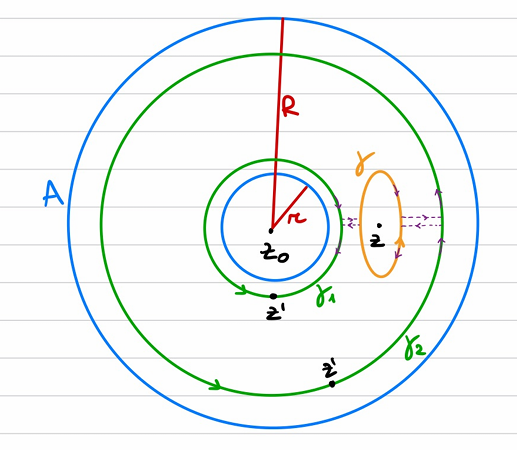
\includegraphics[width=0.5\linewidth]{immagini/Screenshot 2026-02-11 181834.png}
        \label{fig:placeholder}
    \end{figure}
\end{center}
ovvero
\begin{gather}
    \int_{\gamma_2}\frac{dw}{2\pi i}\frac{f(w)}{w - z} - \int_{\gamma_1}\frac{dw}{2\pi i}\frac{f(w)}{w - z} - \int_\gamma\frac{dw}{2\pi i}\frac{f(w)}{w - z} = 0 \notag
\end{gather}
dunque si ottiene
\begin{gather}
    f(z) = \int_{\gamma_2}\frac{dw}{2\pi i}\frac{f(w)}{w - z} - \int_{\gamma_1}\frac{dw}{2\pi i}\frac{f(w)}{w - z} \notag
\end{gather}
per $\gamma_2$ si ha che
\begin{align}
    \frac{1}{w - z} &= \frac{1}{(w - z_0) - (z - z_0)} \notag \\
    &= \frac{1}{w - z_0}\frac{1}{1 - \frac{z - z_0}{w - z_0}} \notag
\end{align}
con $\left|\frac{z - z_0}{w - z_0}\right| < 1$, dunque possiamo utilizzare la serie geometrica per scrivere
\begin{gather}
    \int_{\gamma_2}\frac{dw}{2\pi i}\frac{f(w)}{w - z} = \sum_{n = 0}^\infty\int_{\gamma_2}\frac{dw}{2\pi i}\frac{f(w)}{(w - z_0)^{n + 1}}(z - z_0)^n \notag
\end{gather}
detta parte regolare di $f$. Per $\gamma_1$ si ha
\begin{align}
    \frac{1}{w - z} &= \frac{1}{(w - z_0) - (z - z_0)} \notag \\
    &= \frac{1}{w - z_0}\frac{1}{1 - \frac{z - z_0}{w - z_0}} \notag
\end{align}
tuttavia $\left|\frac{z - z_0}{w - w_0}\right| > 1$, quindi scriviamo
\begin{align}
    \frac{1}{w - z} &= \frac{1}{(w - z_0) - (z - z_0)} \notag \\
    &= \frac{1}{z - z_0}\frac{-1}{1 - \frac{w - z_0}{z - z_0}} \notag
\end{align}
pertanto otteniamo
\begin{align}
    \int_{\gamma_1}\frac{dw}{2\pi i}\frac{f(w)}{w - z} &= -\sum_{n = 1}^\infty\int_{\gamma_1}\frac{dw}{2\pi i}\frac{f(w)}{(w - z_0)^{1-n}}(z - z_0)^{-n} \notag \\
    &= -\sum_{n = -\infty}^{-1}\int_{\gamma_1}\frac{dw}{2\pi i}\frac{f(w)}{(w - z_0)^{n + 1}}(z - z_0)^{n} \notag
\end{align}
dunque
\begin{align}
    f(z) &= \sum_{n = 0}^\infty\int_{\gamma_2}\frac{dw}{2\pi i}\frac{f(w)}{(w - z_0)^{n + 1}}(z - z_0)^n + \sum_{n = -\infty}^{-1}\int_{\gamma_1}\frac{dw}{2\pi i}\frac{f(w)}{(w - z_0)^{n + 1}}(z - z_0)^{n} \notag \\
    &= \sum_{-\infty}^{\infty}d_n(z - z_0)^n \notag
\end{align}
la serie di Laurent convergente uniformemente in ogni corona circolare chiusa contenuta in $A$. \\ \\
\textbf{Definizione:} chiamiamo residuo di $f$ in $z_0$ il coefficiente $d_{-1}$ dello sviluppo in serie di Laurent centrato in $z_0$ della funzione $f$ in una anello contenente solo la singolarità $z_0$ e nessun'altra. \\ \\
\textbf{Proposizione (2.6.1):} sia $z_0$ un polo di ordine $n$ per $f$ olomorfa in $D$, allora si ha che il coefficiente $d_{-k}$, con $k \geq n$, dello sviluppo in serie di Laurent di $f$ centrato in $z_0$ nel primo anello (per ordine) è nullo. \\

\textbf{Dimostrazione:} sia $A = \{z \in D : 0 < |z - z_0| < r\}$ dove $r = d(z_0, \partial D)$, lo sviluppo in serie di Laurent di $f$ centrato in $z_0$ in $A$ è dato da
\begin{gather}
    f(z) = \sum_{-\infty}^{\infty}d_n(z - z_0)^n \notag
\end{gather}
con
\begin{gather}
    d_n = \int_{C_\rho(z_0)} \frac{dw}{2\pi i}\frac{f(w)}{(w - z_0)^{n + 1}} \notag
\end{gather}
per $k \geq n$ si ha
\begin{align}
    d_{-k} = \int_{C_\rho(z_0)} \frac{dw}{2\pi i}f(w)(w - z_0)^{k - 1} \notag
\end{align}
ma per definizione di polo di ordine $n$ esiste un intorno $I$ di $z_0$ tale che
\begin{gather}
    f(z) = g(z)(z - z_0)^n \notag
\end{gather}
per ogni $z \in I$, con $g$ olomorfa in $I$, pertanto $d_{-k}$ diventa l'integrale (a meno di deformare opportunamente il cammino) di una funzione olomorfa su e all'interno di una curva chiusa e per il \textit{teorema di Cauchy - Gaursat} si ha $d_{-k} = 0$, per ogni $k \geq n$.

\newpage
\subsection{Residui}
\textbf{Definizione:} si dice che $f$ ha uno zero di ordine $n$ in $\infty$ se, posto $\eta = 1/z$ la funzione $\phi(\eta) = f(1/\eta) = f(z)$ ha uno zero di ordine $n$ in $\eta = 0$. \\ \\
\textbf{Definizione:} si dice che $f$ ha una singolarità isolata in $\infty$ se, posto $\eta = 1/z$ la funzione $\phi(\eta) = f(1/\eta) = f(z)$ ha una singolarità isolata in $\eta = 0$. \\ \\
\textbf{Definizione:} si dice che $f$ ha un polo di ordine $n$ in $\infty$ se, posto $\eta = 1/z$ la funzione $\phi(\eta) = f(1/\eta) = f(z)$ ha un polo di ordine $n$ in $\eta = 0$. \\ \\
\textbf{Definizione:} si dice che $f$ ha una singolarità essenziale in $\infty$ se, posto $\eta = 1/z$ la funzione $\phi(\eta) = f(1/\eta) = f(z)$ ha una singolarità essenziale in $\eta = 0$. \\ \\
\textbf{Teorema (dei Residui):} sia $f$ olomorfa in $D$ con al massimo $N$ singolarità isolate e sia $\gamma$ una curva chiusa semplice e regolare a tratti, allora
\begin{gather}
    \int_{\gamma}f = 2\pi i \sum_k \mathrm{Res}(f, z_k) \notag
\end{gather}
con $\{z_k\}_{k \in K}$ insieme delle singolarità contenute in $\mathrm{Int}(\gamma)$. \\

\textbf{Dimostrazione:} per ogni $k \in K$ consideriamo una curva chiusa $\gamma_k$ semplice e regolare a tratti percorsa in senso antiorario che contiene solamente $z_k$ e nessun'altra singolarità. Definiamo la curva $\Gamma = \gamma + (-\gamma_1) + \dots + (-\gamma_N)$, per il \textit{primo teorema di Cauchy} si ha
\begin{gather}
    \int_\Gamma f = 0 \notag
\end{gather}
dunque
\begin{gather}
    \int_\gamma f = \sum_k \int_{\gamma_k}f \notag
\end{gather}
\textbf{Teorema (2.7.1):} sia $z_0$ un polo di ordine $n$ per $f$, allora
\begin{gather}
    \mathrm{Res}(f, z_0) = \frac{1}{(n - 1)!}\frac{d^{n-1}}{dz^{n-1}}((z - z_0)^nf(z)) \notag
\end{gather}

\textbf{Dimostrazione:} per definizione di polo di ordine $n$ esiste un intorno $I$ di $z_0$ tale che
\begin{gather}
    f(z) = \frac{g(z)}{(z - z_0)^n} \notag
\end{gather}
per ogni $z \in I$. Allora scelto $\varepsilon > 0$ opportunamente piccolo si ha
\begin{align}
    \mathrm{Res}(f, z_0) &= \int_{C_\varepsilon(z_0)}\frac{dw}{2\pi i}f(w) \notag \\
    &= \int_{C_\varepsilon(z_0)}\frac{dw}{2\pi i}\frac{g(z)}{(z - z_0)^n} \notag
\end{align}
e per il \textit{teorema 2.3.5} si ottiene
\begin{gather}
    \mathrm{Res}(f, z_0) = \frac{1}{(n - 1)!}g^{(n - 1)}(z_0) = \frac{1}{(n - 1)!}\frac{d^{n - 1}}{dz^{n - 1}}((z - z_0)^nf(z)) \notag
\end{gather}
\textbf{Definizione:} sia $f$ una funzione olomorfa con al più singolarità isolate, se $f$ ha una singolarità isolata al punto all'infinito possiamo definire il residuo per $\infty$ come segue
\begin{gather}
    \mathrm{Res}(f, \infty) = \int_{-\gamma}\frac{dw}{2\pi i}f(w) \notag
\end{gather}
con $\gamma$ curva chiusa semplice regolare a tratti e orientata positivamente che contiene tutte le singolarità al finito di $f$. \\ \\
\textbf{Corollario:} segue immediatamente dalla definizione di residuo all'infinito che
\begin{gather}
    \mathrm{Res}(f, \infty) + \sum_k\mathrm{Res}(f, z_k) = 0 \notag
\end{gather}
Osserviamo che il residuo all'infinito è non nullo anche se $f$ è olomorfa all'infinito. \\ \\
\textbf{Lemma (2.7.1):} sia $f$ olomorfa in $D$ e sia $z_0 \in D$ singolarità non eliminabile, allora $f$ non è limitata in un intorno di $z_0$. \\

\textbf{Dimostrazione:} poiché $z_0$ è una singolarità non eliminabile esiste $n > 0$ tale che $d_{-n} \neq 0$, dunque scelto $\varepsilon > 0$ opportunamente piccolo si ha
\begin{align}
    |d_{-n}| &= \left|\int_{C_\varepsilon(z_0)}\frac{dw}{2\pi i}f(w)(w - z_0)^{n - 1}\right| \notag \\
    &< M\varepsilon^n \notag
\end{align}
in particolare per $\varepsilon \rightarrow 0$ deve valere $M \rightarrow \infty$, ovvero $|f|$ non limitato. \\ \\
\textbf{Teorema (Casorati - Weierstrass):} sia $f$ olomorfa in $D$ e sia $z_0$ una singolarità essenziale di $f$, allora si ha che per ogni $\varepsilon > 0$, $\delta > 0$ e $w \in \mathbf{C}$ esiste $z \in D$ tale che se $|z - z_0| < \delta$ si ha $|f(z) - w| < \varepsilon$. \\

\textbf{Dimostrazione:} sia $w \in \mathbf{C}$, supponiamo per assurdo che esiste $\varepsilon > 0$, $\delta > 0$ tale che per ogni $z \in D_\delta(z_0) \setminus \{z_0\}$ si ha $|f(z) - w| > \varepsilon$. Allora la funzione
\begin{gather}
    g(z) = \frac{1}{f(z) - w} \notag
\end{gather}
è olomorfa e limitata in $D_\delta(z_0) \setminus \{z_0\}$, infatti si ha
\begin{gather}
    |g(z)| = \frac{1}{|f(z) - w|} < \frac{1}{\varepsilon} \notag
\end{gather}
dunque per il \textit{lemma 2.7.1} $g$ non può avere un polo o una singolarità essenziale in $z_0$, deve dunque esistere finito
\begin{gather}
    \lim_{z \rightarrow z_0}g(z) = \alpha \in \mathbf{C} \notag
\end{gather}
ma
\begin{gather}
    f(z) = w + \frac{1}{g(z)} \notag
\end{gather}
pertanto
\begin{gather}
    \lim_{z \rightarrow z_0}f(z) = \lim_{z \rightarrow z_0}\left(w + \frac{1}{g(z)}\right) = w + \frac{1}{\alpha} \notag
\end{gather}
tuttavia $z_0$ è una singolarità essenziale per $f$, deve quindi valere
\begin{gather}
    \lim_{z \rightarrow z_0}g(z) = 0 \notag
\end{gather}
sia $j$ l'ordine dello zero $z_0$ per $g$, poiché $g$ è olomorfa in $D_\delta(z_0)$ semplicemente connesso esiste lo sviluppo di Taylor, in particolare si ha
\begin{align}
    g(z) &= \sum_{k = 0}^\infty a_k(z - z_0)^k \notag \\
    &= (z - z_0)^j\sum_{k = j}^\infty a_k(z - z_0)^{k - j} \notag \\
    &= (z - z_0)^jh(z) \notag
\end{align}
per qualche $h$ olomorfa in $D_\delta(z_0)$, ma allora
\begin{gather}
    f = w + \frac{1}{(z - z_0)^jh(z)} \notag
\end{gather}
ovvero $z_0$ polo di ordine $j$ per $f$, ma ciò è un assurdo. \\ \\
\textbf{Lemma (di Jordan):} sia $f$ continua, allora valgono i seguenti risultati: \\
1) Per $a > 0$ si ha
\begin{gather}
    I^+_R = \int_{S^+_R}f(z)e^{iaz} \, dz \rightarrow 0 \notag
\end{gather}
per $R \rightarrow \infty$ se $|f(z)| \rightarrow 0$ uniformemente lungo $S^+_R$ per $R \rightarrow \infty$, cioè se per ogni $R > 0$ esiste $\varepsilon_R > 0$ tale che $|f(Re^{i\phi})| < \varepsilon_R$ per ogni $\phi \in [0, \pi]$. \\ \\
2) Per $a < 0$ si ha
\begin{gather}
    I^-_R = \int_{S^-_R}f(z)e^{iaz} \, dz \rightarrow 0 \notag
\end{gather}
per $R \rightarrow \infty$ se $|f(z)| \rightarrow 0$ uniformemente lungo $S^-_R$ per $R \rightarrow \infty$, cioè se per ogni $R > 0$ esiste $\varepsilon_R > 0$ tale che $|f(Re^{i\phi})| < \varepsilon_R$ per ogni $\phi \in [\pi, 2\pi]$. \\ \\
3) Per $a = 0$ si ha
\begin{gather}
    I_R = \int_{S^\pm_R}f(z) \, dz \rightarrow 0 \notag
\end{gather}
per $R \rightarrow \infty$ se $|Rf(z)| \rightarrow 0$ uniformemente lungo $S^\pm_R$ per $R \rightarrow \infty$. \\

\textbf{Dimostrazione:} per il \textit{teorema di Darboux}: \\
1) si ha che
\begin{align}
    I^+_R &= \int_0^\pi if(Re^{i\phi})Re^{i\phi}e^{iaR\cos\phi}e^{-aR\sin\phi} \, d\phi \notag
\end{align}
dunque
\begin{align}
    |I^+_R| &< \int_0^\pi |f(Re^{i\phi})Re^{-aR\sin\phi}| \, d\phi \notag \\
    &\leq \frac{\pi^2\varepsilon_R}{a} \rightarrow 0 \notag
\end{align}
per $R \rightarrow \infty$, dove si è usata la convessità della funzione $\sin\phi$ per $\phi \in [0, \frac{\pi}{2}]$ per maggiorare l'integrale del termine esponenziale decrescente, in particolare si ha
\begin{gather}
    \sin\phi \leq \frac{2}{\pi}\phi \notag
\end{gather}
per $\phi \in [0, \frac{\pi}{2}]$. \\ \\
2) Analoga. \\
3) si ha che
\begin{align}
    |I_R| &< \int_0^\pi |Rf(Re^{i\phi})| \, d\phi \notag \\
    &\leq \pi\varepsilon_R \rightarrow 0 \notag
\end{align}
per $R \rightarrow \infty$. \\ \\
\subsubsection{Integrali riconducibili a integrale gaussiano}
Calcoliamo l'integrale gaussiano, si ha
\begin{align}
    I_a &= \int_{-\infty}^\infty e^{-ax^2} \, dx \notag
\end{align}
determiniamo il quadrato dell'integrale
\begin{align}
    (I_a)^2 &= \left(\int_{-\infty}^\infty e^{-ax^2} \, dx\right)\left(\int_{-\infty}^\infty e^{-ay^2} \, dy\right) \notag \\
    &= \int_{\mathbf{R}^2} e^{-a(x^2 + y^2)} \, dxdy \notag
\end{align}
poniamo $\rho = x^2 + y^2$ e $\theta = \arctan y/x$, allora
\begin{gather}
    (I_a)^2 = \int_0^\infty\int_0^{2\pi} \rho e^{-a\rho^2} \, d\theta d\rho = 2\pi(-\frac{1}{2a})(e^{-a\rho^2})_0^\infty = \frac{\pi}{a} \notag
\end{gather}
dunque si ottiene $I_a = \sqrt{\frac{\pi}{a}}$. \\ \\
Consideriamo ora
\begin{gather}
    I = \int_{-\infty}^\infty e^{-ax^2 + ipx} \, dx \notag
\end{gather}
si ha che
\begin{gather}
    -ax^2 + ipx = -a\left(x - \frac{ip}{2a}\right)^2 - \frac{p^2}{4a^2} \notag
\end{gather}
pertanto
\begin{gather}
    I = e^{\frac{p^2}{4a^2}}\int_{-\infty - \frac{ip}{2a}}^{\infty - \frac{ip}{2a}} e^{-as^2} \, ds \notag
\end{gather}
consideriamo la seguente curva chiusa $\gamma$ data da
\begin{gather}
    \{\gamma\} = [-R, R] \cup [-R, -R - \frac{ip}{2a}] \cup [-R - \frac{ip}{2a}, R - \frac{ip}{2a}] \cup [R - \frac{ip}{2a}, R] \notag
\end{gather}
percorsa in senso antiorario. La continuazione analitica della funzione integranda è intera in $\mathbf{C}$, dunque l'integrale lungo $\gamma$ è nullo, inoltre per $R \rightarrow \infty$ i termini verticali si annullano e quindi si ottiene
\begin{gather}
    e^{\frac{p^2}{4a^2}}\int_{-\infty - \frac{ip}{2a}}^{\infty - \frac{ip}{2a}} e^{-as^2} \, ds = e^{\frac{p^2}{4a^2}}\int_{-\infty}^{\infty} e^{-as^2} \, ds \notag
\end{gather}
allora si ha
\begin{gather}
    I = e^{\frac{p^2}{4a^2}}\sqrt{\frac{\pi}{a}} \notag
\end{gather}

\newpage
\subsection{Continuazione analitica}
\textbf{Definizione:} sia $f$ olomorfa in $D_f$ e sia $g$ olomorfa in $D_g$ tali che $f(z) = g(z)$ per ogni $z \in D_f \cap D_g$, allora è possibile definire la continuazione analitica di $f$ nel piano complesso come segue
\begin{gather}
    \phi(z) = \begin{cases}
        f(z) \qquad &z \in D_f \\
        g(z) \qquad &z \in D_g
    \end{cases} \notag
\end{gather}
notiamo che la funzione $\phi$ è olomorfa in $D_f \cup D_g$ e $\phi(z) = f(z)$ per ogni $z \in D_f$. Dunque la continuazione analitica è l'estensione di $f$ oltre il suo dominio di analiticità. \\ \\
\textbf{Teorema (2.8.1):} la continuazione analitica di una funzione olomorfa è unica. \\

\textbf{Dimostrazione:} siano $f_1, f_2$ continuazioni analitiche di $f$ in $\tilde{D}$. Allora la funzione $h(z) = f_1(z) - f_2(z)$ è olomorfa in $\tilde{D}$ ed è identicamente nulla in $D$, dato che, per ipotesi, si ha $f(z) = f_1(z) = f_2(z)$ per ogni $z \in D \cap \tilde{D}$. Per il \textit{teorema 2.5.1} sappiamo che gli zeri di una funzione olomorfa sono isolati, dunque deve valere $h(z) = 0$ per ogni $z \in \tilde{D}$, pertanto $f_1(z) = f_2(z)$ per ogni $z \in \tilde{D}$, ovvero la continuazione analitica è unica.

\subsubsection{Metodo di Weierstrass}
Sia $f$ olomorfa in $D$ connesso, sia $z_0 \in D$ e sia $r_0 = d(z_0, \partial D)$, allora per ogni $z \in D_{r_0}(z_0)$ possiamo esprimere $f(z)$ con la sua serie di Taylor, ovvero
\begin{gather}
    f(z) = \sum_{k = 0}^\infty a^{(0)}_k(z - z_0)^k \notag
\end{gather}
Per conoscere il valore di $f(z)$ in un punto $z_e$ esterno a $D_{r_0}(z_0)$ consideriamo una curva $\gamma$ con traccia in $D$ che congiunge $z_0$ a $z_e$. Sia $z_1 \in \{\gamma\}$ e $z_1 \in D_{r_0}(z_0)$, per ipotesi si conosce $f(z_1)$ dato che la serie di Taylor centrata in $z_0$ converge uniformemente in ogni disco chiuso contenuto in $D_{r_0}(z_0)$, pertanto è possibile determinare univocamente i coefficienti $a^{(1)}_k$ per la serie centrata in $z_1$. Quindi si ha
\begin{gather}
    f(z_1) = \sum_{k = 0}^\infty a^{(1)}_k(z - z_0)^k \notag
\end{gather}
inoltre la serie centrata in $z_0$ e la serie centrata in $z_1$ coincidono in $D_{r_0}(z_0) \cap D_{r_1}(z_1)$, ovvero sono una la continuazione analitica dell'altra. Questo procedimento può essere iterato fino a raggiungere $z_e$, ovvero possiamo continuare a ricoprire $D$ con dischi parzialmente sovrapposti fino a raggiungere $z_e$. Ovviamente $z_e$ è un punto fissato dunque basta un numero finito di dischi per raggiungerlo. \\
Nel caso in cui la frontiera del primo disco è composta da punti singolari per $f$ e rende impossibile il proseguimento, essa è detta frontiera naturale di analiticità.

\subsubsection{Metodo del gradiente}
Sia $f$ olomorfa in $D$, sia $z_0 \in D$ e supponiamo di conoscere $f'$ olomorfa in $D$ allora si ha
\begin{gather}
    f(z) = f(z_0) + \int_{\gamma(z_0, z)} f'(z') \, dz' \notag
\end{gather}
dove $\gamma(z_0, z)$ è una curva regolare a tratti con traccia in $D$ che congiunge $z_0$ a $z$. Allora se $f$ ha solo singolarità isolate si ha che $f(z) - f(z_0)$ è indipendente dal cammino $\gamma$ e la continuazione analitica è unica. \\ \\
Questo segue proprio dal fatto che $f'$ ammette una primitiva $f$ che è olomorfa nello stesso dominio $D$. \\
Un controesempio è la funzione $1/z$, olomorfa in $D = \mathbf{C} \setminus \{0\}$, che ammette primitiva un ramo di $\log z$, tuttavia quest'ultima è olomorfa nel piano complesso tagliato (essendo polidroma con punti di diramazione $z = 0$ e $z = \infty$), infatti si ha
\begin{gather}
    \int_{|z| = 1}\frac{1}{z} \, dz \neq 0 \notag
\end{gather}
poiché non ammette primitiva globale. \\ \\
Consideriamo le segue curve
\begin{center}
    \begin{figure}[h]
        \centering
        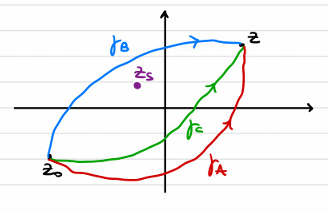
\includegraphics[width=0.5\linewidth]{immagini/Screenshot 2026-02-13 130119.png}
        \label{fig:placeholder}
    \end{figure}
\end{center}
per ipotesi si ha che
\begin{align}
    f_A(z) &= f(z_0) + \int_{\gamma_A} f'(z) \, dz' \notag \\
    f_B(z) &= f(z_0) + \int_{\gamma_B} f'(z) \, dz' \notag \\
    f_C(z) &= f(z_0) + \int_{\gamma_C} f'(z) \, dz' \notag
\end{align}
Poiché $f'$ è olomorfa su e all'interno di $\gamma_A + (-\gamma_B)$ curva chiusa si ha
\begin{align}
    \int_{\gamma_A + (-\gamma_B)} f'(z') \, dz' = 0 \rightarrow f_A(z) = f_C(z) \notag
\end{align}
Mentre si ha
\begin{align}
    \int_{\gamma_A + (-\gamma_B)} f'(z') \, dz' &= f_A(z) - f(z_0) - f_B(z) + f(z_0) \notag \\
    &= f_A(z) - f_B(z) \notag
\end{align}
tuttavia $f'$ ha residuo nullo in $z_s$, infatti sviluppando in serie di Laurent $f$ si vede che $f'$ non ha termine proporzionale a $\frac{1}{z - z_s}$, dunque si ottiene
\begin{gather}
    f_A(z) = f_B(z) \notag
\end{gather}
quindi la continuazione analitica è unica.

\subsubsection{Metodo di Borel}
Sia $f$ olomorfa in $D$ rappresentata dalla serie di Taylor
\begin{gather}
    f(z) = \sum_{k = 0}^\infty a_k(z - z_0)^k \notag
\end{gather}
convergente per ogni $z \in D_R(z_0)$ per qualche $R < \infty$. Sia $\eta_t = t(z - z_0) + z_0$ e sia
\begin{gather}
    \phi_f(z) = \sum_{k = 0}^\infty \frac{a_k}{k!}(z - z_0)^k \notag
\end{gather}
la funzione $\phi_f$ è detta funzione di Borel e ha raggio di convergenza infinito, grazie al fattore $\frac{1}{k!}$. Allora si ha
\begin{align}
    \omega(z) = \int_0^\infty e^{-t}\phi_f(\eta_t) \, dt &= \sum_{k = 0}^\infty \frac{a_k}{k!}(z - z_0)^k\int_0^\infty e^{-t}t^k \, dt \notag \\
    &= \sum_{k = 0}^\infty \frac{a_k}{\cancel{k!}}(z - z_0)^k \cancel{k!} = f(z) \notag
\end{align}
dunque $\omega$ è la continuazione analitica di $f$ nella regione di convergenza dell'integrale. 

\newpage
\subsection{Funzioni polidrome}
Una funzione $f$ è detta polidroma se almeno un punto $z$ del suo dominio di definizione per il quale $f(z)$ può assumere più valori differenti. \\ \\
In generale le funzioni polidrome hanno qualche singolarità isolata e $n > 1$ punti di diramazione. Introducendo un taglio sul piano complesso possono essere trattate come funzioni monodrome. \\ \\
Ci sono varie interpretazioni per le funzioni polidrome. Sia $n$ l'ordine di polidromia di una funzione $f$, allora $f$ può essere interpretata come $n$ funzioni monodrome definite sul piano complesso tagliato. \\
Altrimenti, aggiungendo una dimensione, si può pensare che $f$ sia definita su $n$ superfici di Riemann, tra loro connesso, che tengono conto della discontinuità di $f$.
\begin{center}
    \begin{figure}[h]
        \centering
        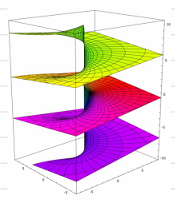
\includegraphics[width=0.3\linewidth]{immagini/Screenshot 2026-02-13 151528.png}
        \label{fig:placeholder}
    \end{figure}
\end{center}
Per determinare se un punto $z_0 \in \mathbf{C}$ è un punto di diramazione per $f$ consideriamo una curva chiusa $\gamma$ che circonda $z_0$, se $z_0$ è un punto di diramazione per $f$ si ha che
\begin{gather}
    \int_\gamma f'(z) \, dz \neq 0 \notag
\end{gather}
ovvero $f$ non è una primitiva di $f'$ in un intorno bucato di $z_0$, ma necessità dell'introduzione di un taglio per esserlo. In particolare questo comporta che la continuazione analitica di $f$ non è unica (per il \textit{metodo del gradiente}). \\ \\
\textbf{Esempio:} consideriamo la funzione $\frac{1}{z}$ olomorfa in $\mathbf{C}^\times$. Si ha che
\begin{gather}
    \int_{|z| = 1}\frac{1}{z} \, dz = 2\pi i \neq 0 \notag
\end{gather}
anche se $\log z$ è una primitiva di $\frac{1}{z}$. Questo perché $\log z$ è una funzione polidroma ed è olomorfa solamente sul piano complesso tagliato, pertanto è una primitiva locale ma non globale di $\frac{1}{z}$. \\ \\
Mentre se consideriamo la funzione $\frac{1}{z^2}$, essa ha come primitiva globale $-\frac{1}{z}$, infatti
\begin{gather}
    \int_{|z| = 1}\frac{1}{z^2} \, dz = 0 \notag
\end{gather}

\newpage
\subsection{Funzioni di operatore}
\textbf{Definizione:} sia $L$ uno spazio lineare $n$-dimensionale, sia $A \in \mathrm{Hom}(L, L)$, lo spettro di $A$ è l'insieme
\begin{gather}
    \sigma(A) = \{z \in \mathbf{C} : \det(z\mathbf{1} - A) = 0\} \notag
\end{gather}
\textbf{Definizione (di Cauchy - Dunford):} sia $L$ uno spazio lineare $n$-dimensionale, sia $A \in \mathrm{Hom}(L, L)$, sia $f$ una funzione olomorfa in $D_f$, allora definiamo la funzione di operatore $f(A)$ come segue
\begin{gather}
    f(A) = \int_{\partial U^+}\frac{dw}{2\pi i}R_A(w)f(w) \notag
\end{gather}
dove $U$ è un aperto tale che $\sigma(A) \subset U$ e $R_A(w) = (w\mathbf{1} - A)^{-1}$, detto risolvente di $A$. Dunque la funzioni di operatore è definita affinché $f$ sia olomorfa nei punti dello spettro di $A$, ovvero deve valere $\sigma(A) \subset D_f$. \\ \\
\textbf{Lemma (2.10.1):} si ha che
\begin{gather}
    R_A(w)R_A(z) = \frac{R_A(z) - R_A(w)}{w - z} \notag
\end{gather}
per ogni $z, w \in \mathbf{C}$ tali che $z, w \not\in \sigma(A)$ e $z \neq w$. \\

\textbf{Dimostrazione:} si ha che
\begin{align}
    \mathbf{1} = (w\mathbf{1} - A)R_A(w)R_A(z)(z\mathbf{1} - A) \notag
\end{align}
ma
\begin{gather}
    \mathbf{1} = \frac{1}{w - z}(w - z)\mathbf{1} = \frac{1}{w - z}[(w\mathbf{1} - A) - (z\mathbf{1} - A)] \notag
\end{gather}
pertanto moltiplicando a destra per $R_A(z)$ e a sinistra per $R_A(w)$ si ottiene la tesi. \\ \\
\textbf{Teorema (2.10.1):} la \textit{definizione di Cauchy - Dunford} soddisfa le seguenti proprietà: \\
1) Se $f_1, f_2, f_1f_2$ sono olomorfe in $D \subset D_1 \cap D_2$ si ha che
\begin{gather}
    f_1(A)f_2(A) = (f_1 \cdot f_2)(A) \notag
\end{gather}
se e solo se
\begin{gather}
    \int_{\partial U^+_1}\frac{dz}{2\pi i}R_A(z)f_1(z)\int_{\partial U^+_2}\frac{dz'}{2\pi i}R_A(z')f_2(z') = \int_{\partial U^+}\frac{dz}{2\pi i}R_A(z)f_1(z)f_2(z) \notag
\end{gather}
dove $U_1, U_2, U$ sono aperti semplicemente connessi tali che $\sigma(A) \subset U_1 \subset D$, $\sigma(A) \subset U_1 \subset D$, $\sigma(A) \subset U \subset D$. \\ \\
2) Se $f(z) = z^n$ si ha $f(A) = A^n$ per ogni $n \in \mathbf{N}$. \\

\textbf{Dimostrazione:} $(1)$ scegliamo $U_1 \subset U_2$, si ha che
\begin{align}
    f_1(A)f_2(A) &= \int_{\partial U^+_1}\frac{dz}{2\pi i}R_A(z)f_1(z)\int_{\partial U^+_2}\frac{dz'}{2\pi i}R_A(z')f_2(z') \notag \\
    &= \int_{\partial U^+_1}\int_{\partial U^+_2}\frac{dzdz'}{(2\pi i)^2}R_A(z)R_A(z')f_1(z)f_2(z') \notag
\end{align}
applicando il risultato del \textit{lemma 2.10.1} si ottiene
\begin{align}
    f_1(A)f_2(A) = \int_{\partial U^+_1}\int_{\partial U^+_2}\frac{dzdz'}{(2\pi i)^2}\frac{R_A(z') - R_A(z)}{z - z'}f_1(z)f_2(z') \notag
\end{align}
tuttavia si ha
\begin{gather}
    \int_{\partial U^+_1}\int_{\partial U^+_2}\frac{dzdz'}{(2\pi i)^2}\frac{f_1(z)}{z - z'}f_2(z')R_A(z') = 0 \notag
\end{gather}
poiché $z'$ è un punto esterno a $U_1$ dunque $\frac{f(z)}{z - z'}$ è olomorfa su e all'interno di $\partial U^+_1$. Mentre, per il \textit{secondo teorema di Cauchy}, si ottiene che
\begin{gather}
    \int_{\partial U^+_1}\int_{\partial U^+_2}\frac{dzdz'}{(2\pi i)^2}\frac{f_2(z')}{z' - z}f_1(z)R_A(z) = \int_{\partial U^+_1}\frac{dz}{2\pi i}f_1(z)f_2(z)R_A(z) \notag
\end{gather}
pertanto si ottiene la tesi. \\ \\
$(2)$ Sia $f(z) = z^n$, per $n = 0$ si ha
\begin{align}
    \int_{\partial U^+}\frac{dz}{2\pi i}(z\mathbf{1} - A)^{-1} &= \int_{C_r(0)}\frac{dz}{2\pi i}\frac{1}{z}\left(\mathbf{1} - \frac{1}{z}A\right)^{-1} \notag \\
    &= \int_{C_r(0)}\frac{dz}{2\pi i}\frac{1}{z}\mathbf{1} = \mathbf{1} \notag
\end{align}
per $r \rightarrow \infty$. Per $n \geq 1$ si ha
\begin{align}
    A^n\mathbf{1} - \int_{\partial U^+}\frac{dz}{2\pi i}z^n(z\mathbf{1} - A)^{-1} &= \int_{\partial U^+}\frac{dz}{2\pi i}(z\mathbf{1} - A)^{-1}(A^n - z^n\mathbf{1}) \notag \\
    &= -\int_{\partial U^+}\frac{dz}{2\pi i}P_{n - 1}(z, A) = 0 \notag
\end{align}
dove si è usato $A^n - z^n\mathbf{1} = (A - z\mathbf{1})P_{n - 1}(z, A)$, con $P_{n - 1}$ polinomio di grado $n - 1$, pertanto si ottiene l'integrale su una curva chiusa di una funzione intera che è nullo per il \textit{teorema di Cauchy - Gaursat}. \\ \\
\textbf{Corollario:} se $f(z) = \sum_{k = 0}^n c_kz^k$ si ha che
\begin{gather}
    f(A) = \sum_{k = 0}^nc_kA^k \notag
\end{gather}

\newpage
\subsection{Proiettori spettrali}
Siano $\lambda_1, \dots, \lambda_m$ gli autovalori di $A$, poiché $\sigma(A) \subset D_f$ si ha che
\begin{gather}
    f(z) = \sum_{n = 0}^\infty a_n(z - \lambda_k)^n \notag
\end{gather}
per ogni $k = 1, \dots, n$. Pertanto usando la \textit{definizione di Cauchy - Dunford} si ottiene
\begin{align}
    f(A) &= \int_{\partial U^+}\frac{dz}{2\pi i}R_A(z)f(z) \notag \\
    &= \sum_{k = 1}^m\int_{\gamma_k}\frac{dz}{2\pi i}R_A(z)f(z) \notag \\
    &= \sum_{k = 1}^m\sum_{n = 0}^\infty a_n\int_{\gamma_k}\frac{dz}{2\pi i}R_A(z)(z - \lambda_k)^n \notag \\
    &= \sum_{k = 1}^m\sum_{n = 0}^\infty a_n E_k^n \notag
\end{align}
dove $\gamma_k$ è una curva chiusa che circonda solamente $\lambda_k$ e $E_k^n$ è detto operatore spettrale di grado $n$ associato all'autovalore $\lambda_k$. \\ \\
\textbf{Teorema (2.11.1):} sia che $E_k^l \cdot E_{k'}^{l'} = \delta_{k \, k'}E_k^{l + l'}$. \\

\textbf{Dimostrazione:} sia $k \neq k'$, scegliamo $\gamma_k$ e $\gamma_{k'}$ che non si intersecano, si ha che
\begin{align}
    E_k^l \cdot E_{k'}^{l'} &= \int_{\gamma_k}\frac{dz}{2\pi i}R_A(z)(z - \lambda_k)^l\int_{\gamma_{k'}}\frac{dz'}{2\pi i}R_A(z')(z' - \lambda_{k'})^l \notag \\
    &= \int_{\gamma_k}\int_{\gamma_{k'}}\frac{dzdz'}{(2\pi i)^2}R_A(z)R_A(z')(z - \lambda_k)^l(z' - \lambda_{k'})^l \notag
\end{align}
e applicando il risultato del \textit{lemma 2.10.1} si ottengono due integrali nulli poiché integrali di funzioni olomorfe su e all'interno di curve chiuse ($\gamma_k$ e $\gamma_{k'}$). \\ \\
Sia $k = k'$, scegliamo $\gamma_k$ contenuta all'interno di $\gamma_{k'}$, si ha che
\begin{align}
     E_k^l \cdot E_{k}^{l'} &= \int_{\gamma_k}\frac{dz}{2\pi i}R_A(z)(z - \lambda_k)^l\int_{\gamma_{k'}}\frac{dz'}{2\pi i}R_A(z')(z' - \lambda_{k})^l \notag \\
    &= \int_{\gamma_k}\int_{\gamma_{k'}}\frac{dzdz'}{(2\pi i)^2}R_A(z)R_A(z')(z - \lambda_k)^l(z' - \lambda_{k})^l \notag
\end{align}
applicando nuovamente il risultato del \textit{lemma 2.10.1} si ottengono due contribuiti dati da
\begin{align}
    \int_{\gamma_k}\int_{\gamma_{k'}}\frac{dzdz'}{(2\pi i)^2}\frac{(z - \lambda_k)^l}{z - z'}(z' - \lambda_k)^lR_A(z') = 0 \notag
\end{align}
poiché la funzione integranda è olomorfa su e all'interno di $\gamma_k$ dato che $z' \in \{\gamma_{k'}\}$. Mentra l'altro termine è
\begin{align}
    \int_{\gamma_k}\int_{\gamma_{k'}}\frac{dzdz'}{(2\pi i)^2}\frac{(z' - \lambda_k)^l}{z' - z}(z - \lambda_k)^lR_A(z) \notag = \int_{\gamma_k}\frac{dz}{2\pi i}(z - \lambda_k)^{l + l'}R_A(z) = E_k^{l + l'} \notag
\end{align}
applicando il \textit{secondo teorema di Cauchy}. Pertanto si ottiene la tesi. \\ \\
\textbf{Osservazione:} se poniamo $f(z) = 1$ si ha che
\begin{align}
    f(A) = \mathbf{1} = \sum_{k = 1}^m E_k^0 \notag
\end{align}
essendo che per $f(z) = 1$ si ha $a_0 = 1$ e $a_n = 0$ per ogni $n > 1$. Se poniamo $f(z) = z$ si ha che
\begin{align}
    f(A) = A = \sum_{k = 1}^m(\lambda_kE_k^0 + E_k^1) \notag
\end{align}
poiché per $f(z) = z$ si ha $a_0 = f(\lambda_k) = \lambda_k$ e $a_1 = 1$. Mentre per $f$ generica tale che $\sigma(A) \subset D_f$ si ha
\begin{align}
    f(A) = \sum_{k = 1}^m\left(f(\lambda_k)E_k^0 + \sum_{n = 1}^{r_k - 1}\frac{f^{(n)}(\lambda_k)}{n!}E_k^n\right) \notag
\end{align}
la somma si tronca a $n = r_k - 1$ poiché per $n = r_k$ si ottiene l'integrale di una funzione olomorfa su e all'interno del cammino di integrazione.

\newpage
\subsection{Caratterizzazione degli operatori diagonalizzabili}
\textbf{Definizione:} è detto indice di autovalore $\lambda_k$ l'intero $\nu_k$ tale che $E_k^{\nu_k} \neq 0$ e $E_k^{\nu_k + 1} = 0$. \\ \\
In generale si ha $\nu_k \leq r_k - 1$, $r_k$ è la molteplicità algebrica dell'autovalore $\lambda_k$, infatti per definizione
\begin{gather}
    E_k^{l} = \int_{C_\varepsilon(\lambda_k)}\frac{dz}{2\pi i}R_A(z)(z - \lambda_k)^l \notag
\end{gather}
dove
\begin{gather}
    R_A(z) = \frac{1}{p_A(z)}C^T(z) \notag
\end{gather}
con $C$ matrice dei cofattori di $z\mathbf{1} - A$ e $p_A$ polinomio caratteristico di $A$. Sappiamo che il polinomio caratteristico ha come radici gli autovalori di $A$, dunque
\begin{gather}
    p_A(z) = \prod_{i = 1}^m(z - \lambda_i)^{r_i} \notag
\end{gather}
Il proiettore $P_k$ non può essere nullo, pertanto $\nu_k \geq 0$ e sostituendo l'espressione per il risolvente di $A$ si ottiene
\begin{gather}
    E_k^l = \int_{C_\varepsilon(\lambda_k)}\frac{dz}{2\pi i}C^T(z)(z - \lambda_k)^{l - r_k}\prod_{i \neq k}(z - \lambda_i)^{r_i} = 0 \notag
\end{gather}
quando $l - r_k \geq 0$, pertanto si ottiene $\nu_k \leq r_k - 1$. \\ \\
\textbf{Definizione:} è detto polinomio minimale il polinomio
\begin{gather}
    \Delta_0(z) = \prod_{k = 1}^m(z - \lambda_k)^{\nu_k + 1} \notag
\end{gather}
\textbf{Teorema (2.12.1):} si ha $\Delta_0(A) = 0$. \\

\textbf{Dimostrazione:} utilizzando i proiettori spettrali si ha
\begin{align}
    \Delta_0(A) &= \sum_{k = 1}^m\left(\cancel{\Delta_0(\lambda_k)}E_k^0 + \sum_{n = 1}^{r_k - 1}\frac{\Delta^{(n)}_0(\lambda_k)}{n!}E_k^n\right) \notag \\
    &= \sum_{k = 1}^m\left(\sum_{n = 1}^{\nu_k}\frac{\Delta^{(n)}_0(\lambda_k)}{n!}E_k^n + \sum_{n = \nu_k + 1}^{r_k - 1}\frac{\Delta^{(n)}_0(\lambda_k)}{n!}E_k^n\right) = 0 \notag
\end{align}
poiché $\Delta^{(n)}_0(\lambda_k) = 0$ per ogni $n \leq \nu_k$ dato che $\lambda_k$ è uno zero di ordine $\nu_k + 1$ di $\Delta_0(z)$, mentre $E_k^n = 0$ per ogni $n \geq \nu_k + 1$ per definizione dell'indice $\nu_k$. \\ \\
\textbf{Teorema (di caratterizzazione degli operatori diagonalizzabili):} sono equivalenti: \\
1) $A$ è diagonalizzabile. \\
2) $E_k^1 = 0$ per ogni $k = 1, \dots, m$. \\
3) $R_A(z)$ ha solo poli semplici. \\
4) $\Delta_0(A) = \prod_{k = 1}^m (A - \lambda_k\mathbf{1}) = 0$ ($\nu_k = 0$ per ogni $k = 1, \dots, m$). \\

\textbf{Dimostrazione:} ($1 \rightarrow 2$) Se $A$ è diagonalizzabile esiste una base di autovettori di $A$ la matrice rappresentativa di $A$ rispetto a tale base è
\begin{gather}
    A = \begin{pmatrix}
        \lambda_1 & & & \\
         & . & & \\
         & & . & \\
         & & & \lambda_m
    \end{pmatrix} \notag
\end{gather}
Allora si ha che
\begin{align}
    R_A(z) &= \frac{1}{\prod_k(z - \lambda_k)}\begin{pmatrix}
        \prod_{k \neq 1}(z - \lambda_k) & & & \\
        & . & & \\
        & & . & \\
        & & & \prod_{k \neq m}(z - \lambda_k)
    \end{pmatrix} \notag \\
    &= \begin{pmatrix}
        (z - \lambda_1)^{-1} & & & \\
        & . & & \\
        & & . & \\
        & & & (z - \lambda_m)^{-1}
    \end{pmatrix} \notag
\end{align}
quindi si ottiene
\begin{align}
    E_k^1 &= \int_{C_\varepsilon(\lambda_k)}\frac{dz}{2\pi i}R_A(z)(z - \lambda_k) \notag = 0 \notag
\end{align}
poiché il fattore $(z - \lambda_k)$ cancella la singolarità in $\lambda_k$, mentre gli altri termini sono olomorfi all'interno di $C_\varepsilon(\lambda_k)$ poiché quest'ultima racchiude solamente $\lambda_k$ e nessun altro autovalore. \\ \\
($2 \rightarrow 3$) Si ha che
\begin{gather}
    E_k^1 = \int_{C_\varepsilon(\lambda_k)}\frac{dz}{2\pi i}R_A(z)(z - \lambda_k) = 0 \notag
\end{gather}
per ogni $k = 1, \dots, m$, allora $R_A(z)$, che può avere solamente poli come singolarità, può essere scritta come
\begin{gather}
    R_A(z) = \frac{G_A(z)}{z - \lambda_k} \notag
\end{gather}
con $G_A$ olomorfa in un intorno di $\lambda_k$ per ogni $k = 1, \dots, m$, ovvero $\lambda_k$ è un polo semplice per ogni $k = 1, \dots, m$. \\ \\
($3 \rightarrow 4$) Poiché $R_A(z)$ ha solo poli semplici si ha che
\begin{gather}
    E_k^1 = \int_{C_\varepsilon(\lambda_k)}\frac{dz}{2\pi i}R_A(z)(z - \lambda_k) = 0 \notag
\end{gather}
per ogni $k = 1, \dots, n$ dato che, per ipotesi, $R_A(z)(z - \lambda_k)$ è olomorfa in un intorno di $\lambda_k$, allora, per definizione, $\nu_k = 0$. La tesi segue dal \textit{teorema 2.12.1}. \\ \\
($4 \rightarrow 1$) Per ipotesi si ha che $\dim\ker \Delta_0(A) = n$, e quindi $\dim\mathrm{Im}\Delta_0(A) = 0$. Ciò comporta che la somma delle molteplicità geometriche degli autovalori $\lambda_k$ è uguale a $n$, infatti si ha
\begin{gather}
    \dim\ker\Delta_0(A) = \dim\ket(A - \lambda_1\mathbf{1}) \oplus \dots \oplus \dim\ker(A - \lambda_m) \notag
\end{gather}
il fatto che il polinomio minimo non abbia radici multiple garantisce il fatto che $A$ non abbia blocchi di Jordan che rendono impossibile la diagonalizzazione.





\newpage
\section{Distribuzioni}
\subsection{Parte principale di Cauchy}
Supponiamo di avere un integrale della forma
\begin{gather}
    I = \int_{-\infty}^{\infty} \frac{f(x)}{x - x_0} \, dx \notag
\end{gather}
con $f$ regolare in $[a, b]$ e $x_0 \in (a, b)$. In generale l'integrale non converge a causa della singolarità in $x_0$, tuttavia utilizzando la parte principale di Cauchy si ha
\begin{gather}
    P\int_{-\infty}^{\infty} \frac{f(x)}{x - x_0} \, dx = \lim_{\varepsilon \rightarrow 0}\int_{-\infty}^{x_0 - \varepsilon} \frac{f(x)}{x - x_0} \, dx + \int_{x_0 + \varepsilon}^{\infty} \frac{f(x)}{x - x_0} \, dx \notag
\end{gather}
l'integrale converge poiché la funzione diverge logaritmicamente in un intorno di $x_0$ e i contributi divergenti si cancellano mutualmente, ovvero si ha che
\begin{gather}
    \int_{x_0 - \varepsilon}^{x_0 + \varepsilon}\frac{f(x)}{x - x_0} \, dx \propto \log|\varepsilon| - \log|\varepsilon| = 0 \notag
\end{gather}
Consideriamo ora lo stesso integrale in $\mathbf{C}$ supponendo che $f(z)$ soddisfi le condizioni del \textit{lemma di Jordan} e che abbia singolarità isolare solo al di fuori dell'asse reale, si ha che
\begin{gather}
    \int_{\Gamma_R} \frac{f(z)}{z - x_0} \, dz = 2\pi i\sum_k \mathrm{Res}(f, z_k) \notag
\end{gather}
dove $z_k$ sono le singolarità di $f$ contenute in $\Gamma_R$ e $\Gamma_R$ è la seguente curva
\begin{center}
    \begin{figure}[h]
        \centering
        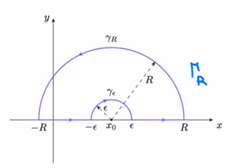
\includegraphics[width=0.35\linewidth]{immagini/Screenshot 2026-02-12 115919.png}
        \label{fig:placeholder}
    \end{figure}
\end{center}
Dimostriamo che al limite per $R \rightarrow \infty$ e $\varepsilon \rightarrow 0$ si ottiene la parte principale di Cauchy. Si ha
\begin{align}
    \int_{\Gamma_R}\frac{f(z)}{z - x_0} \, dz = \left(\int_{-R}^{x_0 - \varepsilon} + \int_{\gamma_\varepsilon} + \int_{x_0 + \varepsilon}^R + \int_{\gamma_R}\right) \frac{f(z)}{z - x_0} \, dz \notag
\end{align}
Il quarto termine del membro di destra si annulla per $R \rightarrow \infty$ poiché per ipotesi $f$ soddisfa le condizioni del \textit{lemma di Jordan}. Il primo e il terzo termine costituiscono la parte principale di Cauchy per $R \rightarrow \infty$. Infine sappiamo che $f$ è olomorfa in $x_0$, dunque esprimiamola in termini della serie di Taylor centrata in $x_0$, allora si ha che il secondo termine diventa
\begin{gather}
    \int_{\gamma_\varepsilon}\frac{f(z)}{z - x_0} \, dz = \sum_{k = 0}^\infty \frac{f^{(k)}(x_0)}{k!}\int_{\gamma_\varepsilon}(z - x_0)^{k - 1} \, dz \notag
\end{gather}
poniamo $z - x_0 = \varepsilon e^{i\phi}$, allora si
\begin{align}
    \int_{\gamma_\varepsilon}\frac{f(z)}{z - x_0} \, dz &= \sum_{k = 0}^\infty \frac{f^{(k)}(x_0)}{k!}\int_\pi^0 i(\varepsilon e^{i\phi})^k \, d\phi \notag
\end{align}
in particolare
\begin{gather}
    \int_\pi^0 i(\varepsilon e^{i\phi})^k \, d\phi = \begin{cases}
        -i\pi \qquad &k = 0 \\
        \varepsilon^n\frac{(1 - e^{i\pi k})}{k} \qquad &k \geq 1
    \end{cases} \notag
\end{gather}
dunque i termini con $k \geq 1$ si annullano per $\varepsilon \rightarrow 0$ e si ottiene
\begin{gather}
    \int_{\gamma_\varepsilon}\frac{f(z)}{z - x_0} \, dz = -i\pi f(x_0) \notag
\end{gather}
per $\varepsilon \rightarrow 0$. Concludiamo che
\begin{gather}
    P\int_{-\infty}^\infty\frac{f(x)}{x - x_0} \, dz = -i\pi f(x_0) + 2\pi i\sum_k\mathrm{Res}\left(\frac{f(z)}{z - x_0}, z_k\right) \notag
\end{gather}

\newpage
\subsection{Distribuzioni come funzioni generalizzate}
Una distribuzione è un funzionale lineare $T : \mathcal{F} \longrightarrow \mathbf{C}$ dove $\mathcal{F}$ è uno spazio di funzioni dette funzioni di test. In generale data una funzione $\phi \in \mathcal{F}$ possiamo scrivere
\begin{gather}
    T(\phi) = \int_{-\infty}^{\infty}f(x)\phi(x) \, dx \notag
\end{gather}
noto come agisce $T$ su un numero abbastanza ampio di funzioni di test $\phi$ è possibile ricostruire la funzione $f$. \\ \\
In generale definiamo due spazi di funzioni di test, scelte in modo tale che abbiamo comportamento più regolare possibile in modo da garantire l'esistenza dell'integrale, in particolare si ha
\begin{gather}
    S(\mathbf{R}) = \{\phi \in C^\infty(\mathbf{R}) : |x|^p\left|\frac{d^q\phi}{dx^q}\right| \rightarrow 0, x \rightarrow 0, \forall p, q\} \notag \\
    D(\mathbf{R}) = \{\phi \in C^\infty(\mathbf{R}) : \phi \text{ ha supporto compatto}\} \notag
\end{gather}
\textbf{Definizione:} si dice che una successioni di funzioni $\{\phi_n\}$ converge uniformemente a $\phi \in \mathcal{F}$ se
\begin{gather}
    \sup_{x \in \mathbf{R}}\left||x|^p\left|\frac{d^q\phi_n}{dx^q}\right| - |x|^p\left|\frac{d^q\phi}{dx^q}\right|\right| \rightarrow 0 \notag
\end{gather}
per $n \rightarrow \infty$ e per ogni $p, q$. \\ \\
Due distribuzioni sono dette uguali se agiscono allo stesso modo su tutte le funzioni di test. Inoltre una distribuzione è detta continua se
\begin{gather}
    \lim_n T(\phi_n) = T(\phi) \notag
\end{gather}
ovvero se il limite commuta con l'operazione $T$, in generale questo accade se la successione converge uniformemente nella regione in cui $T$ opera. \\ \\
Esistono diversi tipi di distribuzioni, se $f$ è localmente integrabile, ovvero l'integrale di $f$ su ogni sottoinsieme compatto converge, si parla di distribuzioni regolari, ad esempio: \\
1) $f(x) = \mathrm{sgn}(x)$ è integrabile in ogni $[a, b]$ compatto e si ha
\begin{gather}
    T_f(\phi) = \int_{-\infty}^0 -\phi(x) \, dx + \int_0^{\infty} \phi(x) \, dx \notag
\end{gather}
2) $f(x) = \theta(x)$ è integrabile in ogni $[a, b]$ compatto e si ha
\begin{gather}
    T_f(\phi) = \int_0^\infty \phi(x) \, dx \notag
\end{gather}
Se invece la distribuzione è non regolare bisogna verificare che è ben definita sulle funzioni di test, in questo caso si parla di distribuzioni singolari, ad esempio: \\
1) La delta di Dirac $\delta_{x_0}(\phi) = \phi(x_0)$, definita come segue in forma integrale
\begin{gather}
    \delta_{x_0}(\phi) = \int_{-\infty}^\infty \delta(x - x_0)\phi(x) \, dx \notag
\end{gather}
2) La funzione $\frac{1}{x}$ non è localmente integrabile intorno a $x = 0$ tuttavia possiamo definire una distribuzione temperata in modo tale da garantire l'esistenza dell'integrale
\begin{gather}
    T(\phi) = \lim_{\varepsilon \rightarrow 0} \int_{-\infty}^{-\varepsilon}\frac{\phi(x)}{x} \, dx + \int_{\varepsilon}^\infty \frac{\phi(x)}{x} \, dx \qquad \left( = P\frac{1}{x}\right) \notag
\end{gather}
\textbf{Proposizione (4.2.1):} vale la seguente identità intesa in senso di distribuzioni
\begin{gather}
    \frac{1}{x \pm i\varepsilon} = P\frac{1}{x} \mp i\pi\delta(x) \notag
\end{gather}

\textbf{Dimostrazione:} sia $\phi$ una funzione di classe $C^1$ integrabile su $\mathbf{R}$, che soddisfa il \textit{lemma di Jordan}. Consideriamo la seguente curva $\gamma_\varepsilon$ data da
\begin{center}
    \begin{figure}[h]
        \centering
        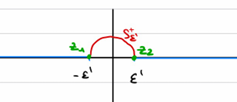
\includegraphics[width=0.5\linewidth]{immagini/Screenshot 2026-02-12 141437.png}
        \label{fig:placeholder}
    \end{figure}
\end{center}
Allora si ha
\begin{align}
    \lim_{\varepsilon \rightarrow 0}\int_{-\infty}^\infty\frac{f(x)}{x \pm i\varepsilon} \, dx &= P\int_{-\infty}^\infty\frac{f(x)}{x} \, dx + \lim_{\varepsilon' \rightarrow 0} \int_{S^\pm_{\varepsilon'}}\frac{f(z)}{z \pm i\varepsilon} \, dz \notag
\end{align}
posto $z = \varepsilon e^{i\phi}$ e quindi $dz = i\varepsilon e^{i\phi}$, si ottiene
\begin{align}
    \lim_{\varepsilon \rightarrow 0}\int_{-\infty}^\infty\frac{f(x)}{x \pm i\varepsilon} \, dx &= P\int_{-\infty}^\infty\frac{f(x)}{x} \, dx + \lim_{\varepsilon \rightarrow 0} \int_{S^\pm_{\varepsilon'}}\frac{f(z)}{z \pm i\varepsilon} \, dz \notag \\
    &= P\int_{-\infty}^\infty\frac{f(x)}{x} \, dx \mp i\pi f(0) \notag
\end{align}
è necessario deformare la curva perché non è ben definito l'integrale altrimenti, anche se il limite è esterno all'operazione di integrale.

\newpage
\subsection{Operazioni sulle distribuzioni}
Molte operazioni che possono essere eseguite sulle funzioni possono essere definite anche per le distribuzioni. \\
1) Cambio di variabili: sia $g(x) = f(u(x))$ con $u$ di classe $C^\infty$ strettamente monotona, allora si ha che
\begin{gather}
    T_g(\phi) = \int_{-\infty}^\infty f(u(x))\phi(x) \, dx = \int_{-\infty}^\infty f(y)\frac{\phi(u^{-1}(y)}{u'(u^{-1}(y))} \, dy \notag
\end{gather}
avendo posto $y = u(x)$ e quindi $dy = u'dx$. \\ \\
2) Traslazione: sia $x_0 \in \mathbf{R}$ vogliamo traslare $x_0 \rightarrow x_0 + a$ per qualche $a \in \mathbf{R}$. Poniamo
\begin{gather}
    \delta_{x_0} \circ T_a(\phi) = \delta_{x_0}(\phi \circ T^{-1}_a) = \int_{-\infty}^\infty \delta(x - x_0)\phi(x - a) \, dx = \phi(x_0 - a) \notag
\end{gather}
3) Riscalare: sia $\lambda \in \mathbf{R}$ vogliamo riscalare $x_0 \rightarrow \lambda x_0$. Poniamo
\begin{gather}
    \delta_{x_0}(\phi) \circ R_\lambda(\phi) = \delta_{x_0}\left(\frac{\phi \circ R^{-1}_\lambda}{|\lambda|}\right) = \frac{\phi(0)}{|\lambda|} \notag
\end{gather}
4) Derivata: definiamo la derivata di distribuzione utilizzando la serie di funzioni che converge alla distribuzione. In particolare poniamo
\begin{gather}
    \int_{-\infty}^{\infty}\frac{d\phi}{dx}f(x) \, dx = \lim_n \int_{-\infty}^\infty\frac{d\phi_n}{dx}f(x) \, dx \notag
\end{gather}
e integrando per parti si ottiene
\begin{align}
    \lim_n \int_{-\infty}^\infty\frac{d\phi_n}{dx}f(x) \, dx &= \cancel{\lim_n \phi_n(x)f(x)|_{-\infty}^\infty} - \int_{-\infty}^\infty\phi_n(x)f'(x) \, dx \notag \\
    = -\int_{-\infty}^\infty\phi(x)f'(x) \, dx \notag
\end{align}
La somma di distribuzioni è sempre definita usando una rappresentazione in successione per le distribuzioni. Il prodotto di distribuzioni in generale non è ben definito ma ci sono alcune eccezioni, ad esempio
\begin{align}
    \delta_x\delta_{x - a}(\phi) = \lim_n \int_{-\infty}^\infty\delta(x)\phi(x)\frac{n}{\sqrt{\pi}}e^{-n(x - a)^2} \, dx = \phi(0)\frac{n}{\pi}e^{-na^2} \rightarrow \phi(0) \notag
\end{align}
per $n \rightarrow \infty$. Mentre se $a = 0$ non è definita poiché il limite diverge. \\ \\
\textbf{Teorema (4.3.1):} si ha $\delta_x = \frac{d\theta}{dx}$ in senso di distribuzioni, su $\mathbf{R}$ e su un intervallo generico $[a, b]$. \\

\textbf{Dimostrazione:} sia $f$ una funzione di test, su $\mathbf{R}$ si ha
\begin{align}
    \int_{\mathbf{R}}\frac{d\theta}{dx}f(x) \, dx &= [\theta(x)f(x)]_{\infty}^{\infty} - \int_{\mathbf{R}}\theta(x)f'(x) \, dx \notag \\
    &= - \int_0^\infty f'(x) \, dx = f(0) \notag
\end{align}
Su $[a, b]$, $a < 0$ e $b > 0$ si ha
\begin{align}
    \int_a^b\frac{d\theta}{dx}f(x) \, dx &= [\theta(x)f(x)]_a^b - \int_a^b\theta(x)f'(x) \, dx \notag \\
    &= f(b) - \int_0^b f'(x) \, dx = f(0) \notag
\end{align}
per $a > 0, b > 0$ si ha
\begin{align}
    \int_a^b\frac{d\theta}{dx}f(x) \, dx &= [\theta(x)f(x)]_a^b - \int_a^b\theta(x)f'(x) \, dx \notag \\
    &= f(a) - f(b) - \int_a^bf'(x) \, dx = 0 \notag
\end{align}
per $a < 0, b < 0$ si ha
\begin{align}
    \int_a^b\frac{d\theta}{dx}f(x) \, dx &= [\theta(x)f(x)]_a^b - \int_a^b\theta(x)f'(x) \, dx = 0 \notag
\end{align}

\subsubsection{Proprietà della delta di Dirac}
\textbf{Teorema:} valgono le seguenti proprietà per la delta di Dirac:
\begin{gather}
    1. \qquad \delta(ax) = \frac{1}{|a|}\delta(x) \notag
\end{gather}
per ogni $a \in \mathbf{R}$.
\begin{gather}
    2. \qquad (x - x_0)^{2l}\delta(a(x - x_0)^{2l + 1}) = \frac{\delta(x - x_0)}{|a|(2l + 1)} \notag
\end{gather}
per ogni $l \in \mathbf{N}$.
\begin{gather}
    3. \qquad x\delta(x^3) \text{ o } \delta(x^3) \notag
\end{gather}
non hanno senso poiché non ben definite.
\begin{gather}
    4. \qquad \delta(g(x)) = \sum_{j = 1}^N\frac{\delta(x - x_j)}{|g'(x_j)|} \notag
\end{gather}
per ogni $g$ con $N$ zeri semplici $x_1, \dots, x_N$.
\begin{gather}
    5. \qquad (x - x_0)^{2l}\delta(F(x)) = \frac{(2l!)\delta(x - x_0)}{|F^{(2l + 1)}(x_0)|} \notag
\end{gather}
per ogni $F$ con un zero di ordine $2l + 1$ in $x_0$.
\begin{gather}
    6. \qquad x\delta(x^2) = 0 \notag
\end{gather}
se la funzione di test ha parità definita. \\

\textbf{Dimostrazione:} proseguendo per ordine: $(1)$ sia $a > 0$, allora si ha
\begin{align}
    \int_{-\infty}^\infty \delta(ax)f(x) \, dx &= \int_{-\infty}^\infty \delta(y)f\left(\frac{y}{a}\right) \, \frac{dy}{a} = \frac{f(0)}{a} \notag
\end{align}
ponendo $y = ax$. Mentre
\begin{align}
    \int_{-\infty}^\infty \delta(-ax)f(x) \, dx &= -\int_\infty^{-\infty} \delta(y)f\left(-\frac{y}{a}\right) \, \frac{dy}{a} \notag \\
    &= \int_{-\infty}^\infty \delta(y)f\left(-\frac{y}{a}\right) \, \frac{dy}{a} = \frac{f(0)}{a} \notag
\end{align}
$(2)$ Sia $l \in \mathbf{N}$ si ha che
\begin{align}
    \int_{-\infty}^\infty (x - x_0)^{2l}\delta((x - x_0)^{2l + 1})f(x) \, dx &= \int_{-\infty}^\infty \delta(y)f\left(x_0 + y^{\frac{1}{2l + 1}}\right) \, \frac{dy}{2l + 1} \notag \\
    &= \frac{f(x_0)}{2l + 1} \notag
\end{align}
$(3)$ Facendo sempre il cambio di variabili $y = x^3$ si ottiene un integrale divergente. \\
$(4)$ Si ha che
\begin{align}
    \int_{-\infty}^\infty \delta(g(x))f(x) \, dx &= \sum_j\int_{x_j - \varepsilon}^{x_j + \varepsilon}\delta(g'(x_j)(x - x_j) + o(x - x_j))f(x) \, dx \notag \\
    &= \sum_j\frac{\delta(x - x_j)}{|g'(x_j)|} \notag
\end{align}
per il punto $(1)$. \\
$(5)$ Segue immediatamente dalla $(1)$ e dalla $(4)$. \\
$(6)$ Si ha che $\delta(x^2)$ è sempre rappresentata dal limite di una successioni di funzioni pari $\phi_n$, dunque si ha
\begin{gather}
    \int_{-\infty}^{\infty} x\delta(x^2)f(x) \, dx = \int_{-\infty}^0 x\delta(x^2)f(x) \, dx + \int_0^\infty x\delta(x^2)f(x) \, dx \notag
\end{gather}
poniamo $u = x^2$, dunque $dx = \frac{du}{2\sqrt{u}}$, inoltre
\begin{gather}
    \begin{cases}
        x = \sqrt{u} \qquad &x > 0 \\
        x = -\sqrt{u} \qquad &x < 0
    \end{cases} \notag
\end{gather}
pertanto otteniamo
\begin{align}
    \int_{-\infty}^{\infty} x\delta(x^2)f(x) \, dx &= -\int_0^\infty \delta(u)f(-\sqrt{u}) \, \frac{du}{2} + \int_0^\infty \delta(u)f(\sqrt{u}) \, \frac{du}{2} \notag \\
    &= -\int_{-\infty}^\infty \delta(u)f(-\sqrt{u}) \, \frac{du}{4} + \int_{-\infty}^\infty \delta(u)f(\sqrt{u}) \, \frac{du}{4} \notag \\
    &= \frac{1}{4}(f(0^+) - f(0^-)) = 0 \notag
\end{align}
poiché $f(0^+) = f(0^-)$ se $f$ è pari e $f(0^\pm) = 0$ se $f$ è dispari. \\ \\
\textbf{Teorema (rappresentazione della delta di Dirac):} sia $p$ una qualsiasi funzione pari, assolutamente integrabile in $\mathbf{R}$ e normalizzata, allora si ha che
\begin{gather}
    \delta(x) = \lim_n p_n(x) = \lim_n np(nx) \notag
\end{gather}

\textbf{Dimostrazione:} sia $f$ continua in $[a, b]$ e sia
\begin{align}
    F_n(x_0) = \int_a^b p_n(x - x_0)f(x) \, dx = n\int_a^b p(n(x - x_0))f(x) \, dx \notag
\end{align}
poniamo
\begin{gather}
    t = n(x - x_0) \qquad dt = ndx \notag
\end{gather}
allora si ha
\begin{align}
    F_n(x_0) = \int_{n(a - x_0)}^{n(b - x_0)}p(t)f(t/n + x_0) \, dt \notag
\end{align}
se $x_0 \not\in (a, b)$ si ha che
\begin{gather}
    \begin{cases}
        n(a - x_0), n(b - x_0) \rightarrow -\infty \qquad &x_0 > b \\
        n(a - x_0), n(b - x_0) \rightarrow \infty \qquad &x_0 < a
    \end{cases} \notag
\end{gather}
per $n \rightarrow \infty$ e quindi si ha
\begin{gather}
    \lim_n F_n(x_0) = 0 \notag
\end{gather}
se $x_0 \in (a, b)$ si ha che
\begin{gather}
    \lim_n F_n(x_0) = \int_{-\infty}^\infty p(t)f(x_0) \, dt = f(x_0) \notag
\end{gather}
infatti si ha che
\begin{gather}
    \phi_n(t) = p(t)f(t/n + x_0) \notag
\end{gather}
può essere maggiora, infatti
\begin{gather}
    |\phi_n(t)| \leq M|p(t)| \notag
\end{gather}
dove $M = \max_{x \in [a, b]}|f(x)|$, che esiste poiché $f$ è continua in un compatto. Quindi si può applicare il teorema della convergenza dominata di Lebesgue e si ottiene la tesi.

\subsubsection{Rappresentazione integrale della theta}
Si ha che la distribuzione $\theta$ può essere ottenuta come segue
\begin{gather}
    \theta(x) = \lim_{\varepsilon \rightarrow 0}\int_{-\infty}^\infty \frac{e^{ixt}}{t - i\varepsilon} \, dt \notag
\end{gather}
infatti la funzione integranda soddisfa le condizioni del \textit{lemma di Jordan}, pertanto per $x > 0$ si ha
\begin{align}
    \int_{-\infty}^\infty \frac{e^{ixt}}{t - i\varepsilon} \, dt &= \mathrm{Res}\left(\frac{e^{ixt}}{t - i\varepsilon}, i\varepsilon\right) \notag \\
    &= e^{-x\varepsilon} \rightarrow 1 \notag
\end{align}
per $\varepsilon \rightarrow 0$. Per $x < 0$ si ha
\begin{gather}
    \int_{-\infty}^\infty \frac{e^{ixt}}{t - i\varepsilon} \, dt = 0 \notag
\end{gather}
poiché la funzione integranda non ha singolarità nel semipiano inferiore.

\newpage
\section*{Appendice}
\textbf{Teorema (di Gauss - Green):} sia $S \subset \mathbf{R}^2$ una superficie e sia $F \in C^1(S, \mathbf{R}^2)$, allora
\begin{gather}
    \int_{\partial S^+}F \cdot d\mathbf{s} = \iint_{S}\left(\frac{\partial f_2}{\partial x} - \frac{\partial f_1}{\partial y}\right) \, dxdy \notag
\end{gather}
\textbf{Lemma (di Gauss):} se $F = (f(x, y), 0)$ si ha
\begin{gather}
    \int_{\partial S^+}F \cdot d\mathbf{s} = -\int_S \frac{\partial f}{\partial y} \, dxdy \notag
\end{gather}
Analogamente, se $F = (0, f(x, y))$ si ha
\begin{gather}
    \int_{\partial S^+}F \cdot d\mathbf{s} = \int_S \frac{\partial f}{\partial x} \, dxdy \notag
\end{gather}
 
\end{document}
